%!TEX root = ../chapter1.tex
%******************************
%	 Results 
%******************************

\section{Single-cell RNA sequencing of murine CD4\plus{} T cells}

\begin{wrapfigure}{r}{0.5\textwidth}
\centering    
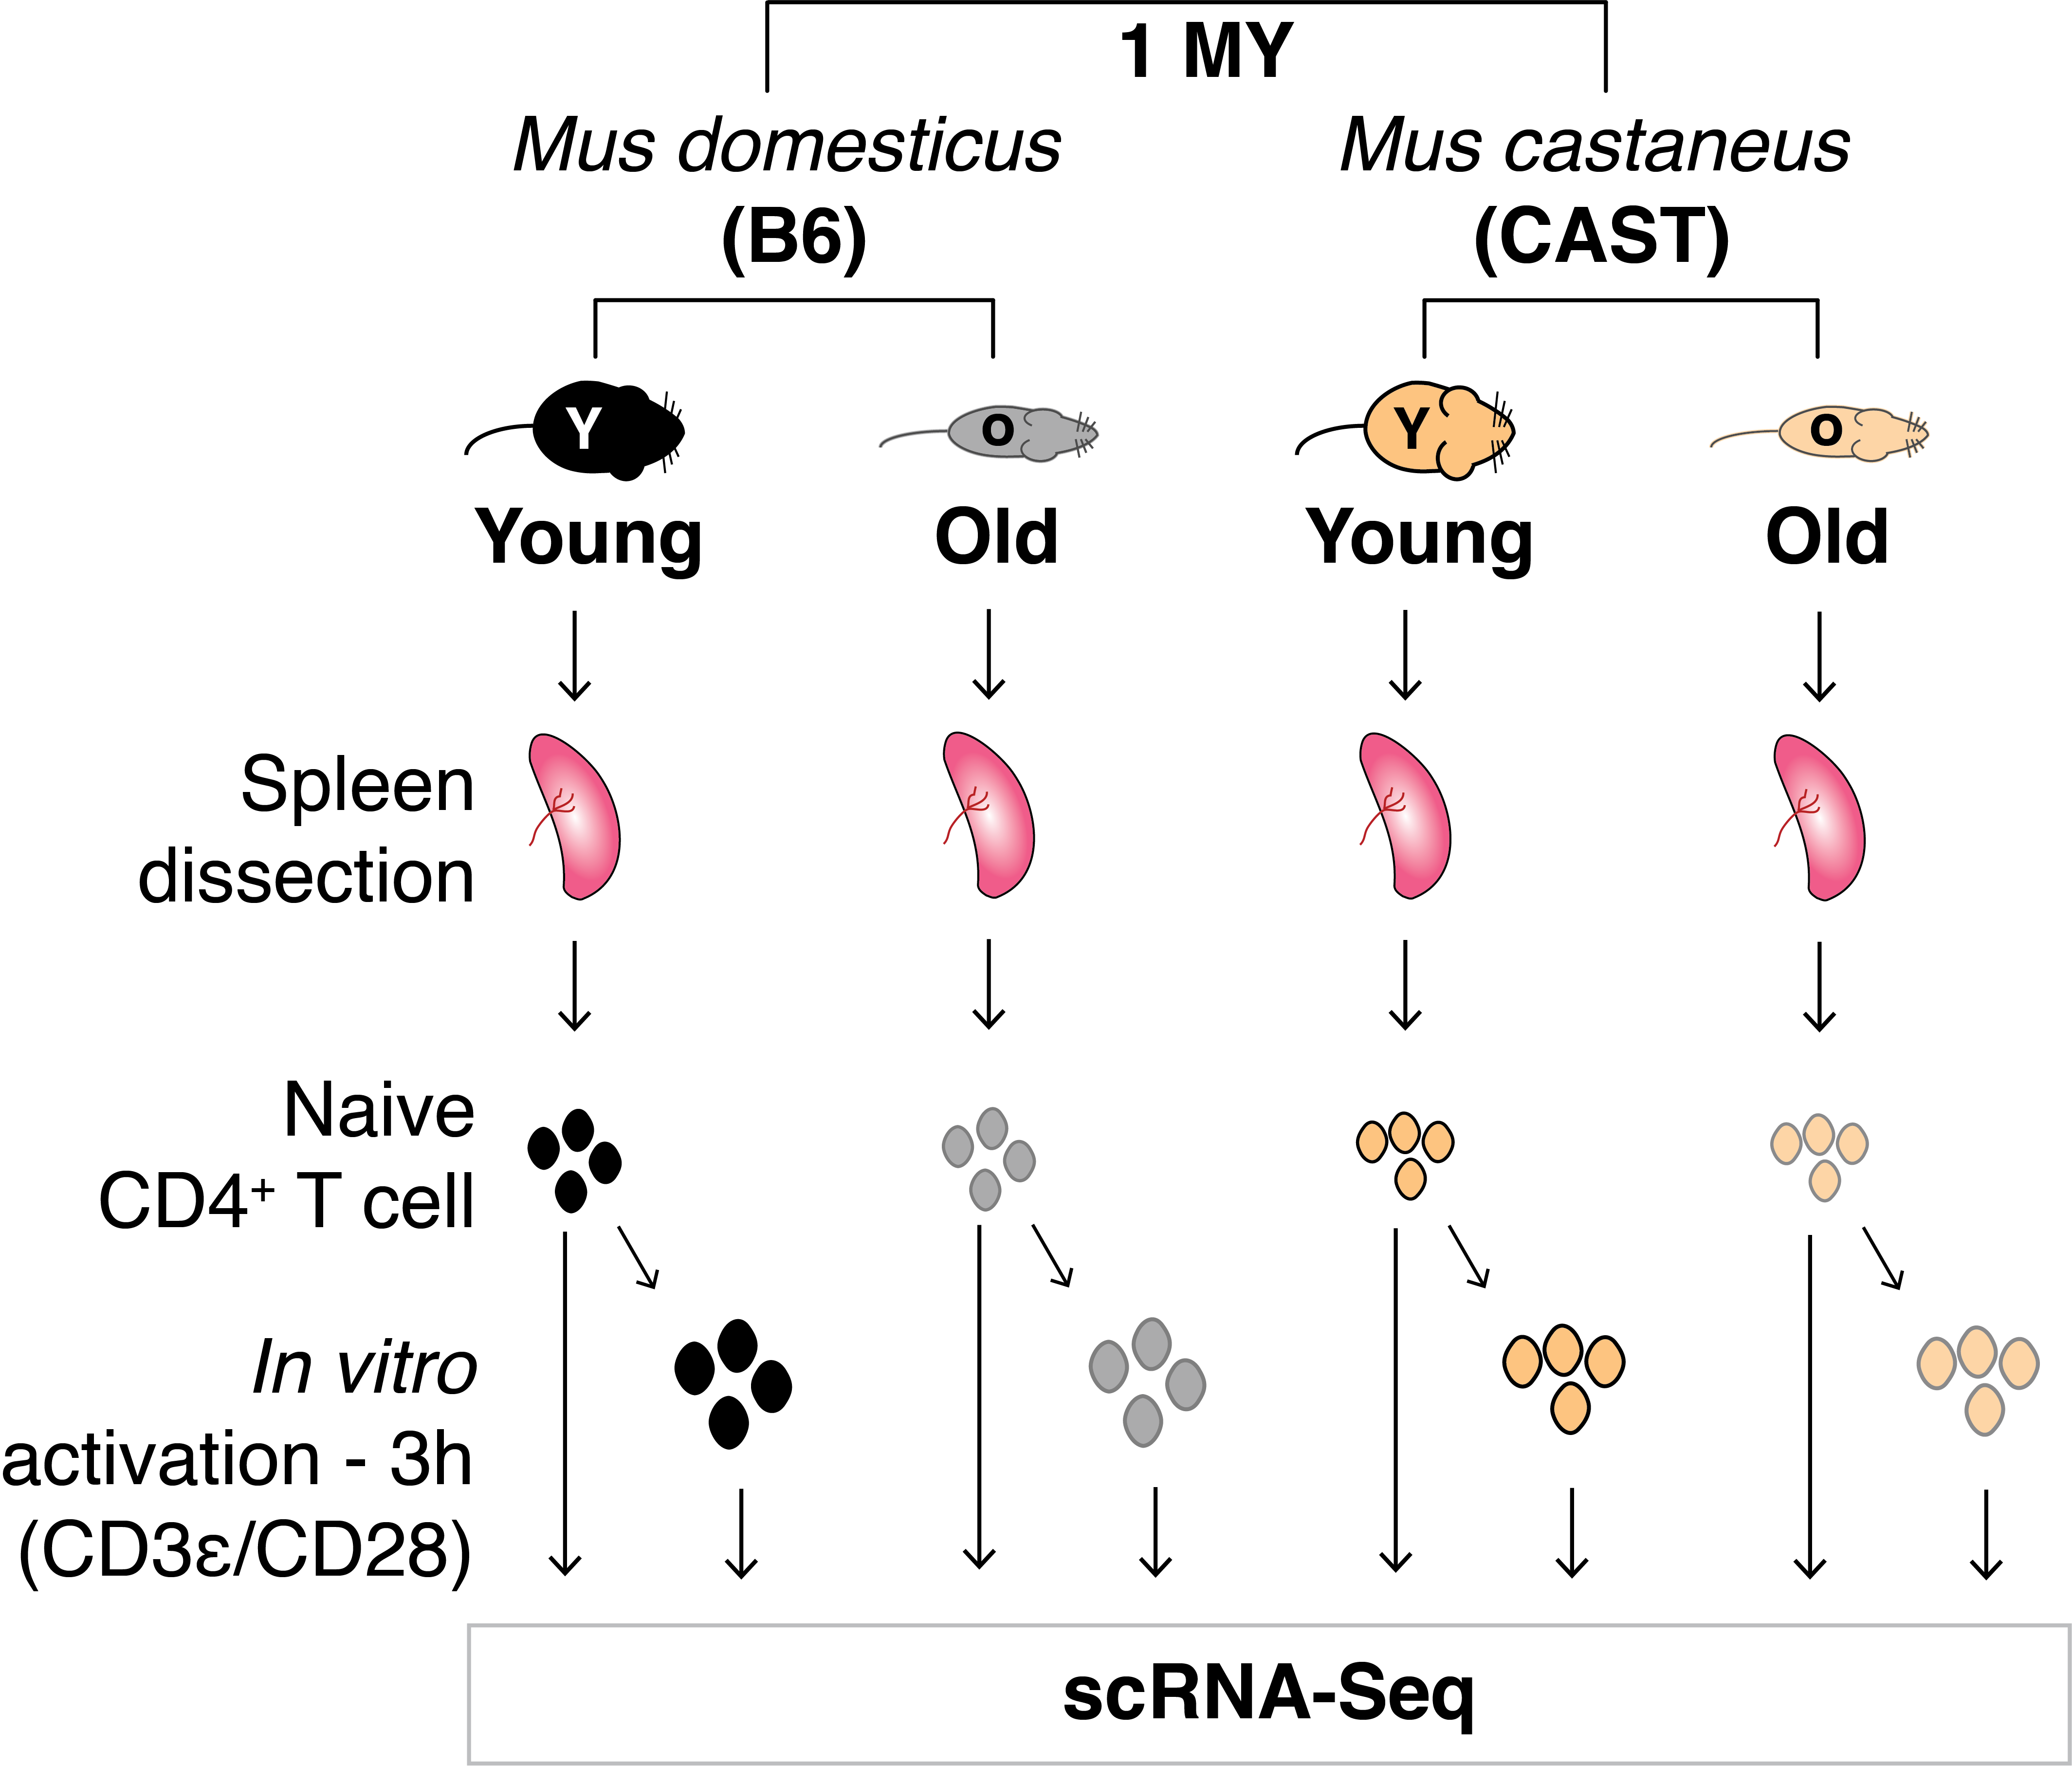
\includegraphics[width=0.48\textwidth]{Fig_1.png}
\caption[scRNA-Seq of CD4\plus{} T cells from young and old mice.]{\textbf{scRNA-Seq of unstimulated and activated CD4\plus{} T cells from young and old B6 and CAST animals.} \\
Single cells were isolated from spleens of young (~3 month) and old (~21 month) individuals of two related mouse sub-species (\textit{Mus musculus domesticus}, B6; \textit{Mus musculus castaneus}, CAST). Isolated cells were subjected to single-cell mRNA sequencing (scRNA-Seq) before or after 3 hours of \textit{in vitro} activation using anti-CD3\textepsilon{} and CD28 coated plates.}
\label{fig1:overview}
\end{wrapfigure}

To assess transcriptional changes of the immune activation programme during ageing, we isolated CD4\plus{} T cells from healthy individuals of two inbred mouse sub-species separated by 1 million years of divergence: the reference C57BL/6J, \gls{B6} and CAST/EiJ, \gls{CAST}. Furthermore, we isolated CD4\plus{} T cells from young (~3 months) and old (~21 months) individuals. To characterise their gene expression programme, we performed scRNA-Seq using the C1 Fluidigm system \textbf{(Fig.~\ref{fig1:overview})}. The two sub-species have similar lifespans \citep{Yuan2011}, and CAST mice showed the hallmarks of normal organismal ageing as observed in B6 mice \citep{Rodwell2004}. All mice were healthy at the time of experiments. To assess different CD4\plus{} T cell compartments, we assayed cell populations isolated with different levels of purity. First, we isolated all unstimulated CD4\plus{} T cells from spleens of old and young animals. Secondly, we highly purified naive CD4\plus{} T cells and \gls{EM} CD4\plus{} T cells. For simplification and clarity, purified unstimulated CD4\plus{} T cells will be named naive; stimulated cells will be named activated. Highly purified naive CD4\plus{} T cells will be named FACS-purified naive CD4\plus{} T cells and highly purified EM CD4\plus{} T cell will be referred to as FACS-purified EM CD4\plus{} T cells. For each species/condition, scRNA-Seq experiments were independently performed using cells isolated from two individuals. Full experimental methods can be found in \textbf{Appendix \ref{appA.1}}.

\newpage

\subsection{Experimental strategy}

\subsubsection{Unstimulated CD4\plus{} T cells}

\begin{wrapfigure}{rt}{0.5\textwidth}
\centering    
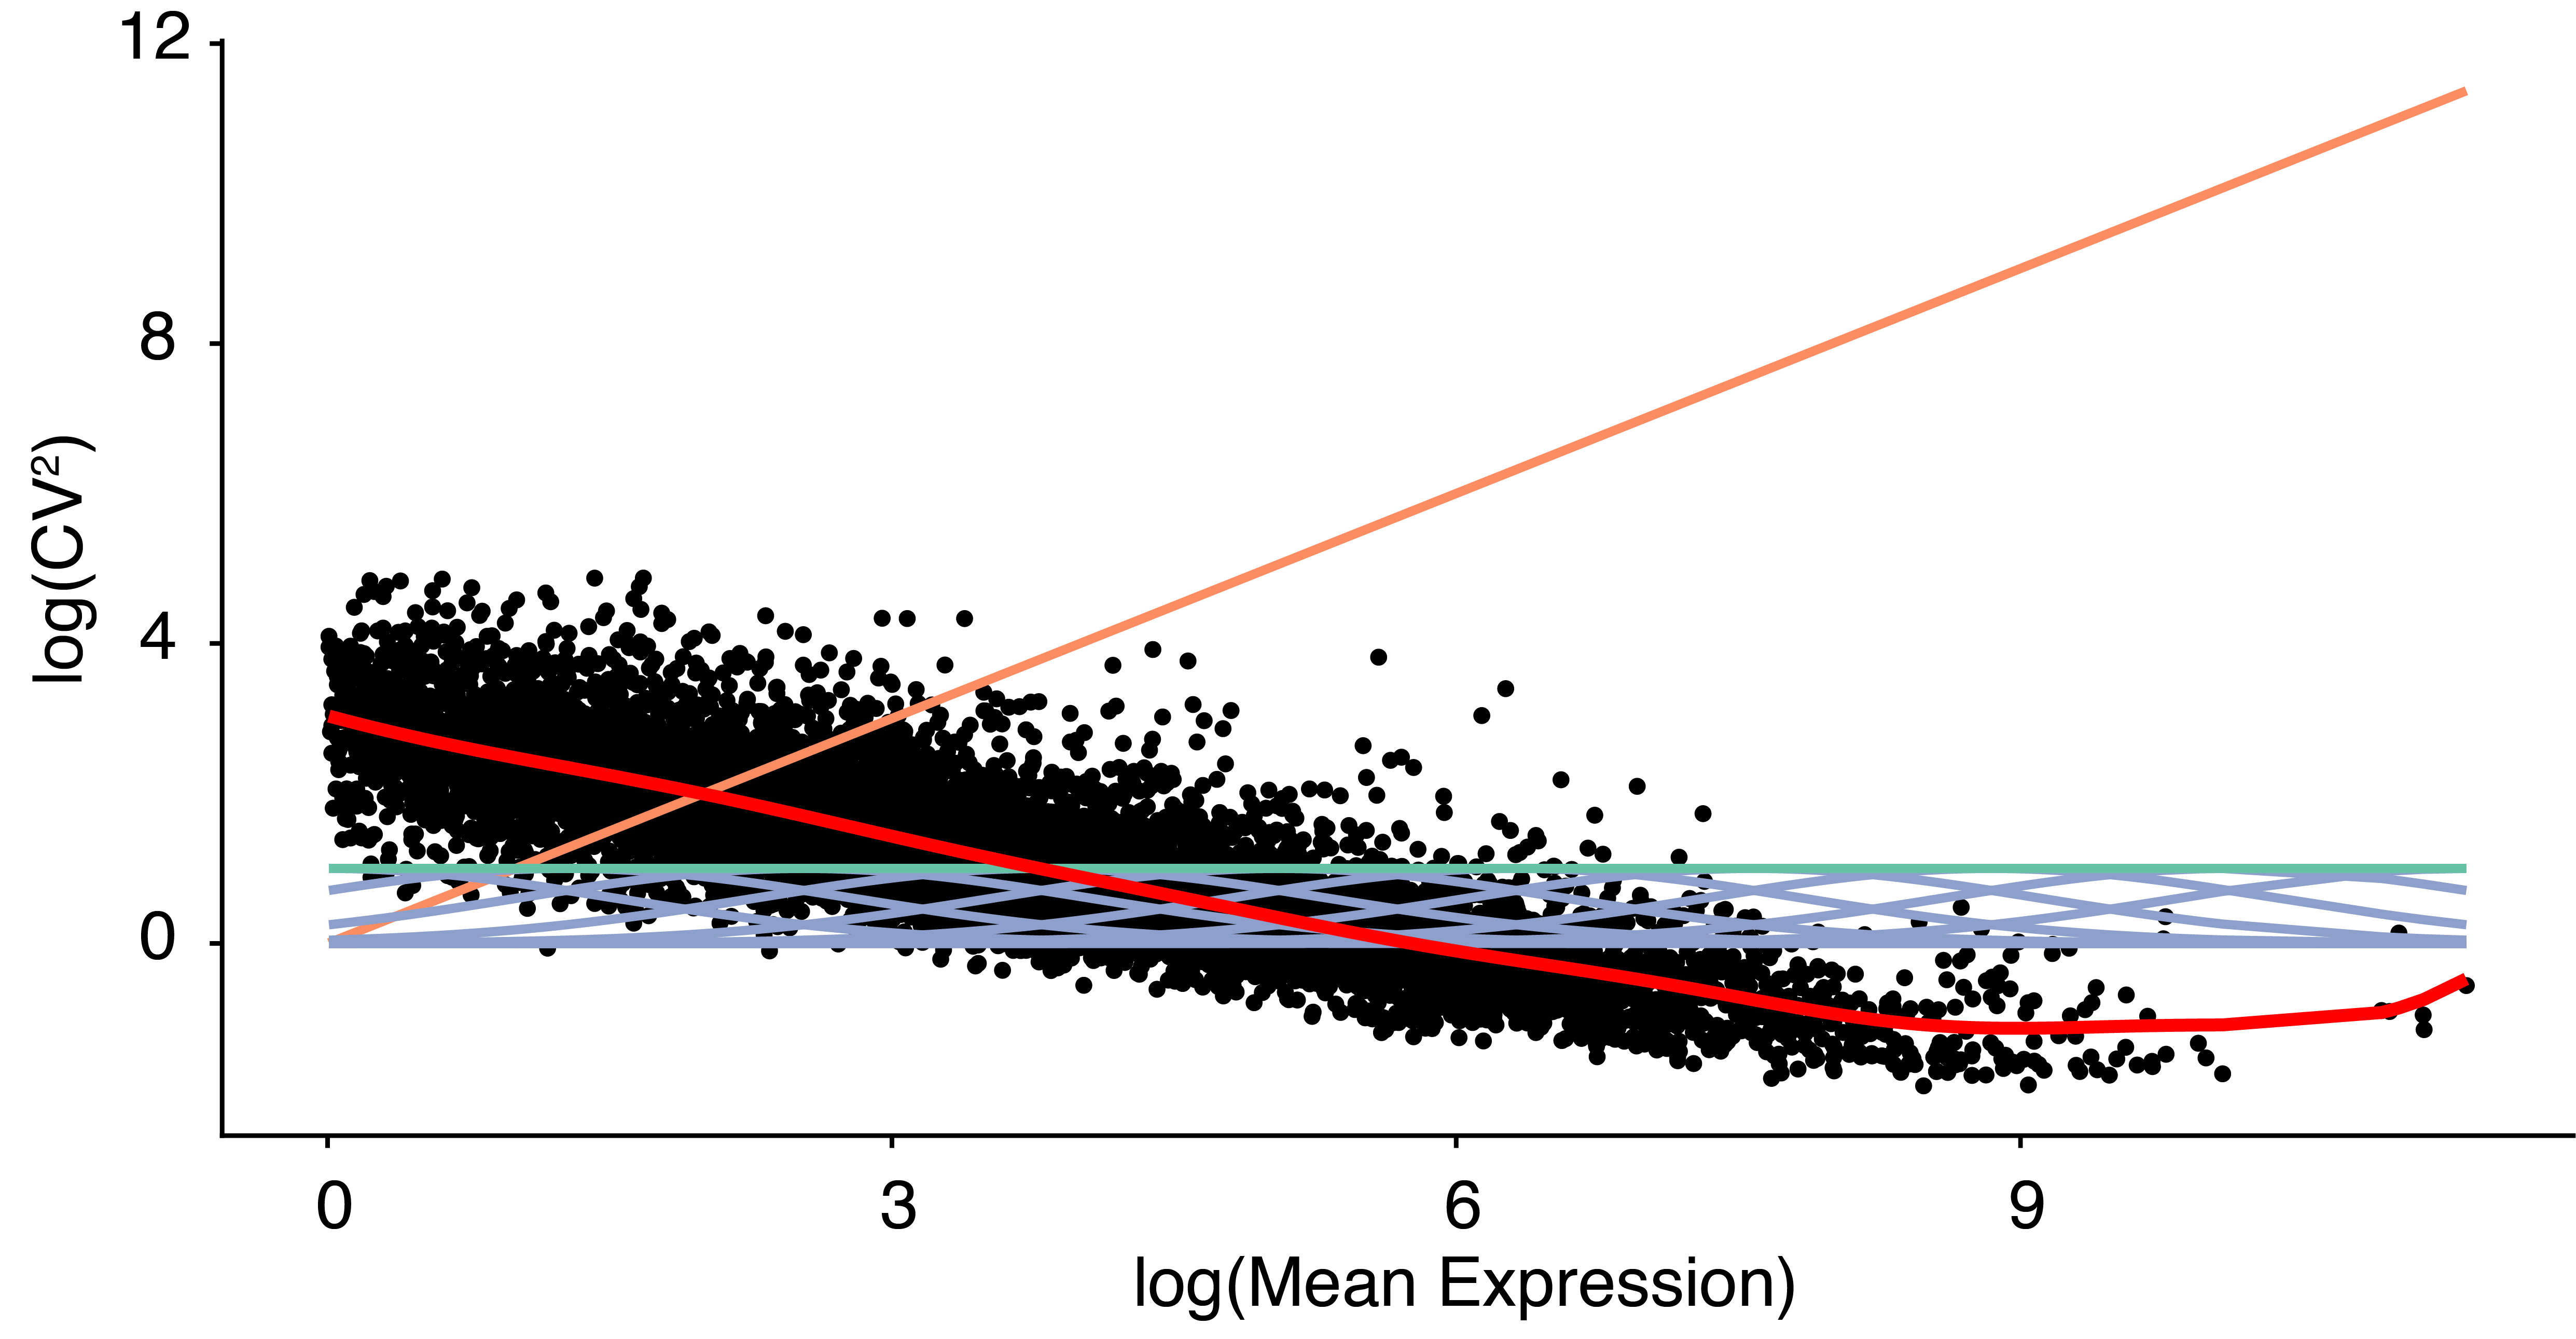
\includegraphics[width=0.48\textwidth]{Fig_2.png}
\caption[FACS of naive and effector memory CD4\plus{} T cells]{\textbf{FACS of naive and effector memory CD4\plus{} T cells.} \\
Gating Strategy: lymphocytes were gated by the use of \gls{FSC} and \gls{SSC}. Cell doublets were excluded according to area and height of FSC (FSC-A/FSC-H). Dead cells were removed using viability dye. \Gls{PD1}\plus{} CD4\plus{} T cells were excluded and PD-1-ve CD4\plus{} T cells were further separated into naive and EM CD4\plus{} T cell subsets according to their CD44 and CD62L expression. Cells with a mature CD24$^\text{lo}$ Qa2$^\text{hi}$ phenotype were then gated from naive and EM subsets and CD69\plus{} cells were removed. From \citep{Martinez-jimenez2017}. Reprinted with permission from AAAS.}
\label{fig1:FACS}
\vspace{-50mm}
\end{wrapfigure}

Unstimulated CD4\plus{} T cells were purified from dissociated mouse spleens using cell strainers, cell separation media and a \gls{MACS} CD4\plus{} CD62L\plus{} T Cell Isolation Kit (see \textbf{Appendix \ref{appA.1:isolation}}). 

\subsubsection{Naive and effector memory CD4\plus{} T cells}

Naive and EM CD4\plus{} T cells were purified from spleens of both young and old BL6 mice by FACS.  Briefly, spleens were harvested from both young and old animals and single cell suspensions were obtained by meshing through a cell strainer. B cells were depleted from cell suspensions by MACS using CD19 microbeads and red blood cells were lysed with red blood cell lysis buffer. The enriched cell fraction was then stained with Fixable eFluor 780 viability dye following Fc receptor blocking with TruStain fcXTM and subsequent staining with a panel of fluorescence-conjugated antibodies against CD4, CD44, CD62L, CD24, Qa2, CD69 and PD-1.  Stained cells were immediately sorted using FACS with the stringent gating strategy described in \textbf{Fig.~\ref{fig1:FACS}} (see \textbf{Appendix \ref{appA.1:FACS}}). 

\newpage

\subsubsection{Activation of CD4\plus{} T cells}

96-well plates were coated with anti-CD3\textepsilon{} and anti-CD28 antibodies (see \textbf{Appendix \ref{appA.1:isolation}}). After this, naive and FACS-purified naive cells were seeded into these plates at a density of 80,000-120,000 cells/ml, and then cultured in a total volume of 100 \textmu{}l media that did not contain cytokines or additional antibodies. With this strategy, CD4\plus{} T cells are purely activated but do not commit to a T helper cell fate \citep{Stubbington2015, Zhu2010}.

\subsubsection{scRNA-Seq using the Fluidigm C1 system}

Unstimulated and activated CD4\plus{} T cells were loaded on a 5–10 \textmu{}m Auto Prep IFC to capture single cells using the C1 Single cell Auto Prep System (Fluidigm). All IFCs were visually inspected, and wells with multiple cells or cell debris were marked as low quality. Upon cell capture, reverse transcription and cDNA amplification were performed using the SMARTer PCR cDNA Synthesis Kit and the Advantage 2 PCR Kit. ERCC spike-in RNA (1 \textmu{}L diluted at 1:50,000) was added to the C1 lysis mix. All capture sites were included for the RNA-Seq library preparation (see \textbf{Appendix \ref{appA.1:RNA-Seq}}).

\subsection{Computational strategy}
\label{sec1:computational}

\subsubsection{Read alignment to reference genomes}

For all capture sites, read alignment to reference genomes was performed using \emph{gsnap} with default parameters, while supplying splice-site positions \citep{Wu2010a}. Samples taken from B6 were mapped against the mouse reference \gls{GRCm38}. CAST samples were aligned against the \emph{Mus musculus castaneus de novo} genome assembly (\url{ftp://ftp-mouse.sanger.ac.uk/REL-1509-Assembly/}, now available on Ensembl \url{ftp://ftp.ensembl.org/pub/release-92/fasta/mus_musculus_casteij/dna/}), which was used under an advance access agreement (\url{ftp://ftp-mouse.sanger.ac.uk/REL-1509-Assembly/README}). Gene annotation for B6 was taken from the GRCm38 reference; gene annotation for CAST was taken from the newly constructed \emph{Mus musculus castaneus} assembly (\url{http://hgwdev.cse.ucsc.edu/~ifiddes/mouse_genomes_data/}, version 0.2, now available at \url{ftp://ftp.ensembl.org/pub/release-92/gtf/mus_musculus_casteij/}). Additionally, since mitochondrial genes and certain immune genes (e.g., CD28) are absent from the \emph{Mus musculus castaneus} annotation used, and since high mitochondrial gene expression is a well-established signature of low-quality single-cell transcriptome profiles \citep{Ilicic2016}, we also mapped CAST reads against GRCm38 and used the B6 annotation solely for the mitochondrial genes. Gene expression counts were obtained using \emph{HTSeq} with default options \citep{Anders2014}. Only genes with orthologs in both species were considered for downstream analysis. 

\subsubsection{Quality control and filtering}

We visually inspected the cell-capture sites in each C1 IFC using 40x magnification lensing to ensure precise capture of single cells \textbf{(Fig.~\ref{fig1:QC}A and B)}. Low-quality cells were computationally filtered using the following quality control criteria:\\
The percentage of reads mapping to annotated genomic regions was compared to the percentage of reads mapping to ERCC spike-ins. Cells with low genomic reads (< 20\%) and/or high ERCC reads (> 50\%) were excluded \textbf{(Fig.~\ref{fig1:QC}C)}. Additionally, cells with  a low total number of mapped reads (< 1,000,000) were excluded. To exclude possible doublets and dying cells, capture sites with > 3000 or < 1250 detected genes were removed \textbf{(Fig.~\ref{fig1:QC}D and E)}. Next, cells with more than 10\% or less than 0.5\% of mitochondrial reads were excluded \textbf{(Fig.~\ref{fig1:QC}F)}. These quality filtered cells were tested for possible batch effects by computing a PCA on both replicates. We detect no batch effect since cells from the two individuals are overlapping (see \textbf{Fig.~\ref{fig1:QC}G} for an example of naive and activated CD4\plus{} T cells of young B6).\\

To control for biological contamination, known markers of lymphocytes were used to filter cells: CD19\plus{}/H2-Aa\plus{} B cells as well as CD8\plus{} T cells were removed \textbf{(Fig.~\ref{fig1:QC}H)}. Finally, we visualised naive and activated CD4\plus{} T cells using \gls{tSNE} and detect a strong grouping depending on the activation status. Here, non-activated T cells that were meant to be activated were removed from downstream analysis \textbf{(Fig.~\ref{fig1:QC}I)}. Read counts were normalised using the BASiCS package \citep{Vallejos2015} incorporating spike-in reads for technical noise estimation. Prior to normalisation, genes not expressed in at least 3 cells (rpm > 20) were filtered out. Similarly, ERCC spike-ins were removed if not detected in the data set.

\newpage

\begin{figure}[!hb]
\centering
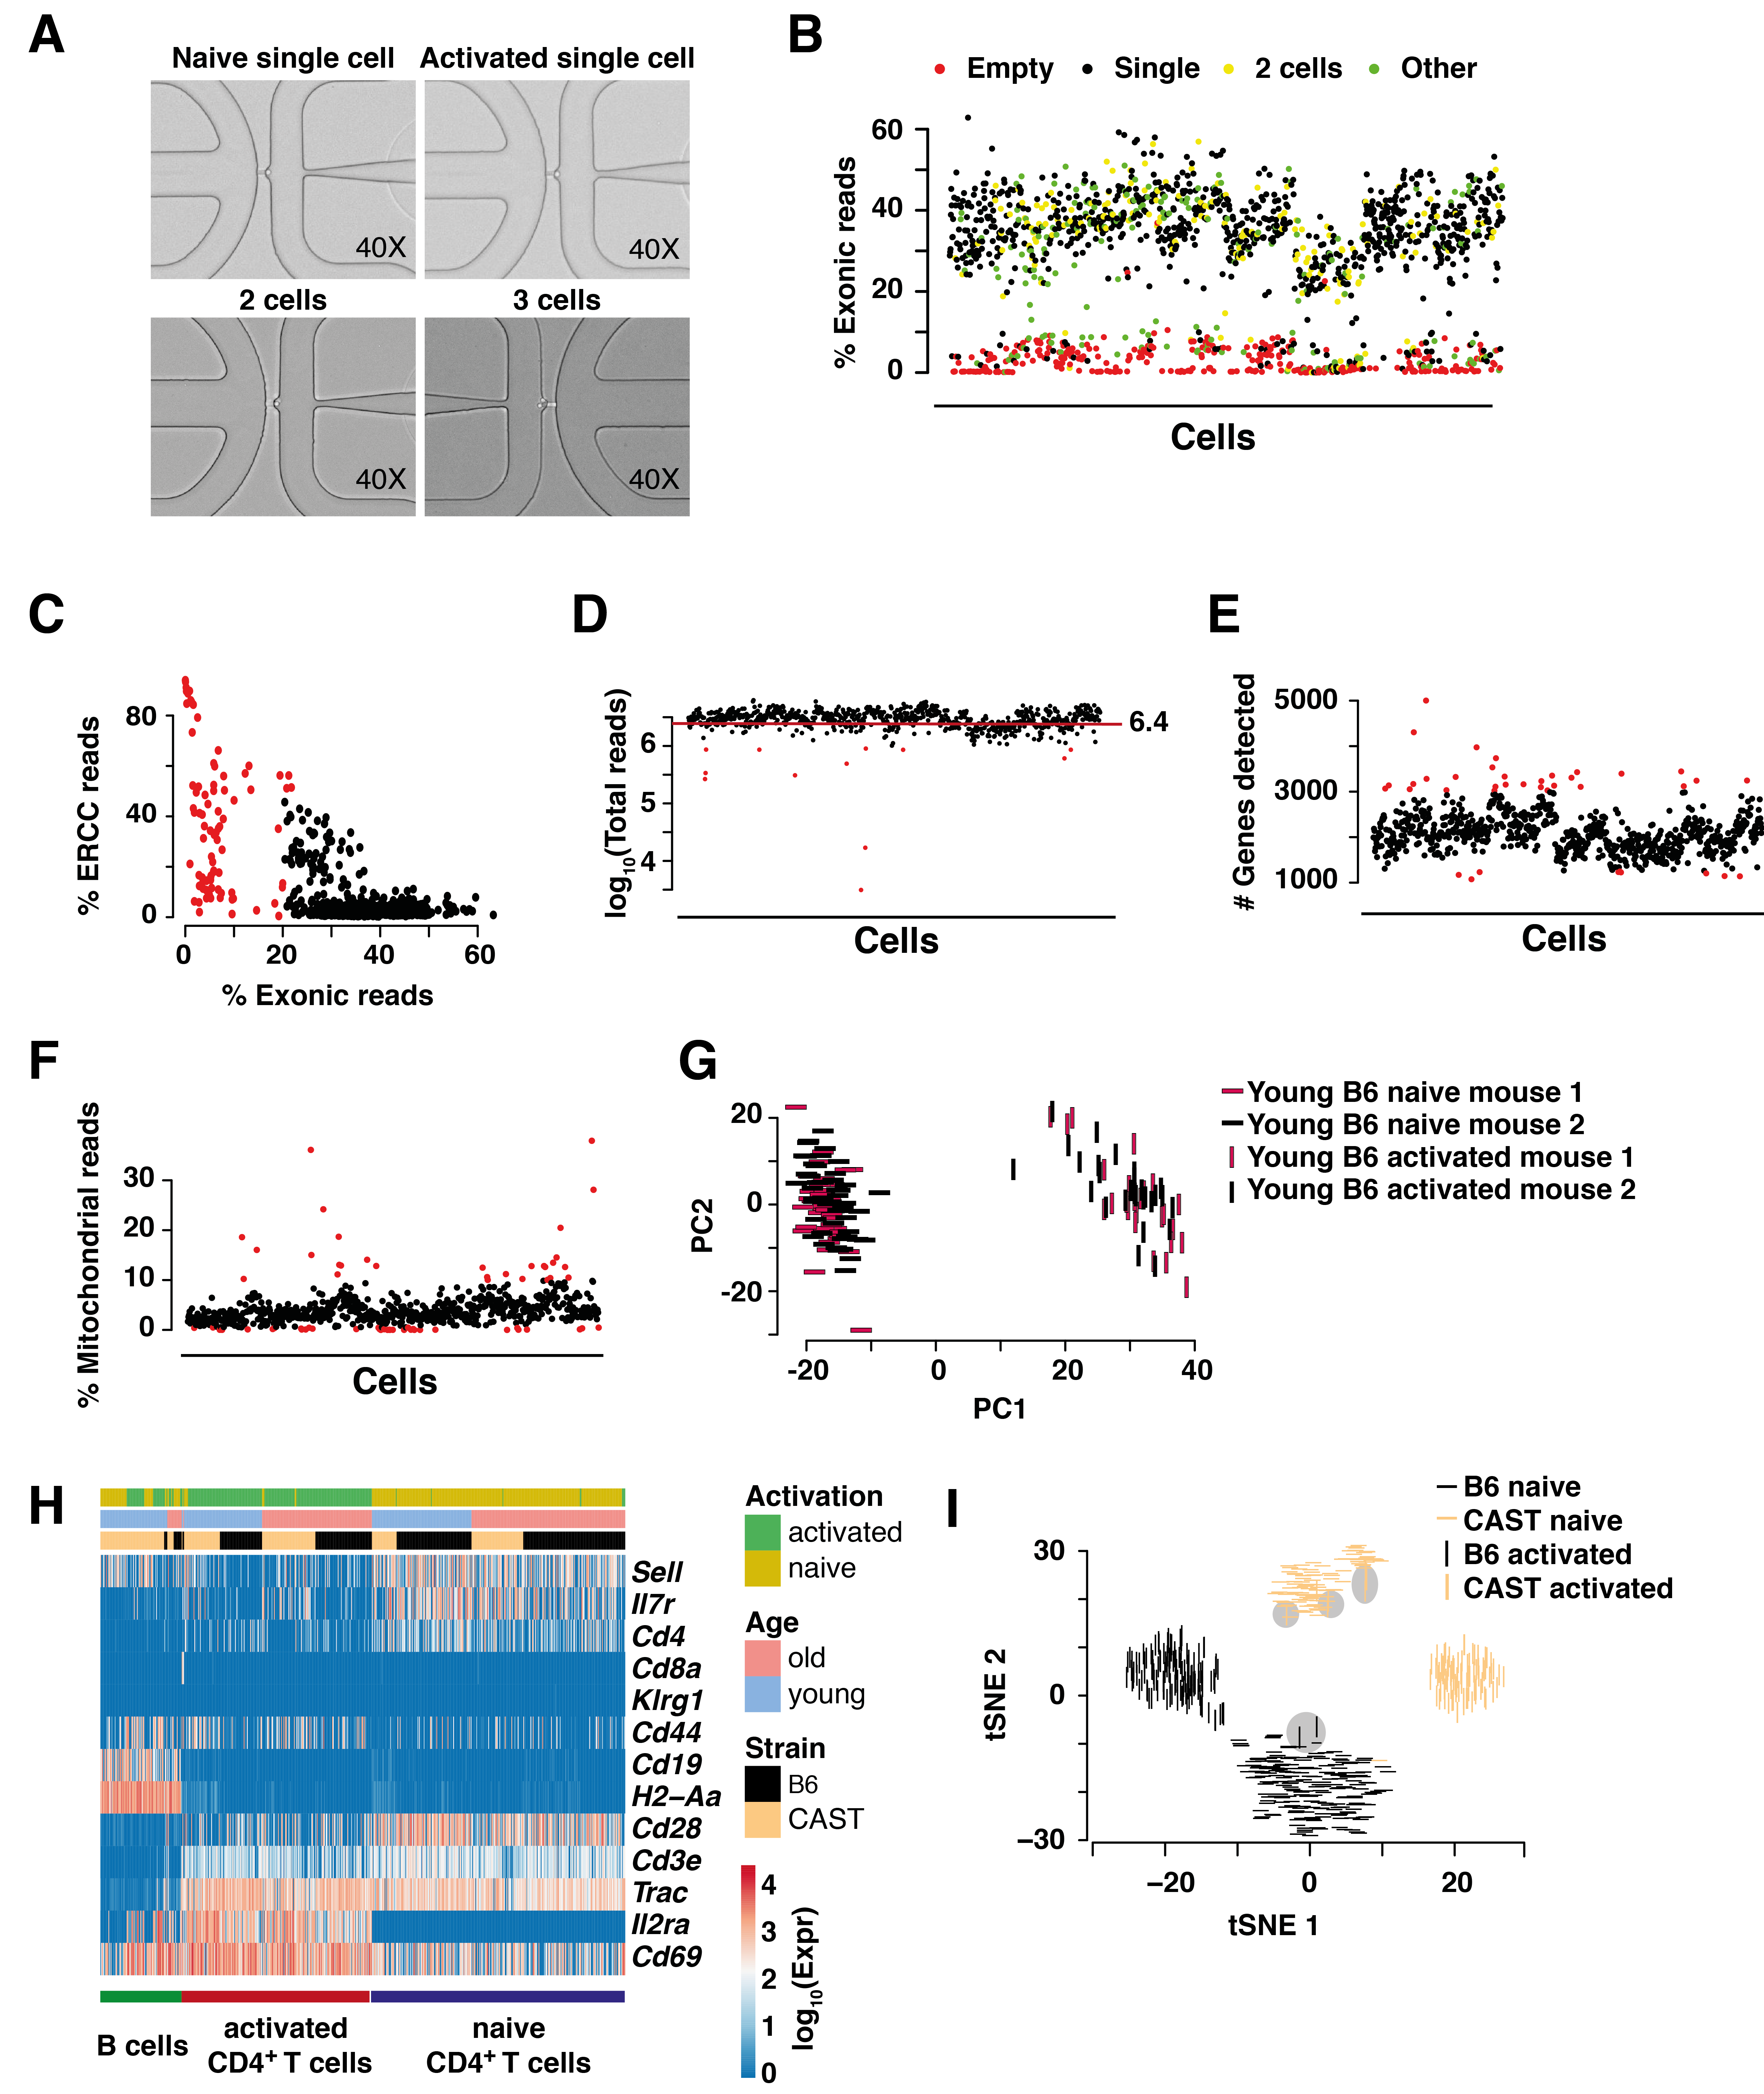
\includegraphics[width=\textwidth,trim={0 4cm 0 0},clip]{Fig_3.png}
\caption[Quality control of isolated CD4\plus{} T cells]{\textbf{Quality control of isolated CD4\plus{} T cells (Full legend on next page).}\\}
\label{fig1:QC}
\end{figure}

\newpage

\captionsetup[figure]{list=no}
\addtocounter{figure}{-1}   
\captionof{figure}{\textbf{Quality control of isolated CD4\plus{} T cells (continued).}\\
\textbf{(A)} Visual inspection of captured cells at 40x magnification in IFCs (C1, Fluidigm) allows manual removal of empty capture sites, and capture sites holding multiple cells or debris, \textbf{(B)} Percentage of reads mapping to exonic regions displayed for naive and activated CD4\plus{} T cells. Black dots: single cells, yellow dots: 2 cells, red dots: empty wells, green dots: debris, multiple cells, etc., \textbf{(C)} Removal of cells with less than 20\% of mapped exonic reads and more than 50\% of ERCC spike-in reads (red dots), \textbf{(D)} Cells with less than 1 million mapped reads were excluded from downstream analysis (red dots),  \textbf{(E)} Cells with more than 3000 or less than 1250 genes were excluded in the analysis (red dots), \textbf{(F)} Cells with more than 10\% or less than 0.5\% of mitochondrial reads were excluded from downstream analysis (red dots), \textbf{(G)} Naive and activated cells isolated from young B6 animals (replicates) were coloured batch-specifically. 4 batches from 2 mice: naive and activated from mouse 1 (white bars), naive and activated from mouse 2 (black bars). Naive condition is represented in horizontal bars and activated condition in vertical bars, \textbf{(H)} Data set was filtered for immune markers to exclude B cell and CD8\plus{} T cell contamination. Cells in columns were labelled based on their activation state (naive in beige, activated in green), their age (old in red, young in blue), and the species of the animals (B6 in black, CAST in yellow). Cells were ordered based on their \textit{\gls{H2-Aa}} and \textit{\gls{Il2ra}} expression, \textbf{(I)} tSNE visualisation allowed the removal of not fully activated cells (indicated in grey circles). Cells were labelled based on their activation state (naive: horizontal bar, activated: vertical bar) and the species of the animals (B6 in black, CAST in yellow). From \citep{Martinez-jimenez2017}. Reprinted with permission from AAAS.}
\captionsetup[figure]{list=yes}

\subsubsection{BASiCS parameter estimation using transcriptomes of CD4\plus{} T cells}
\label{sec1:BASiCS}

To quantify and assess changes in mean expression and expression variability, we used the Bayesian hierarchical framework BASiCS introduced in \textbf{Section \ref{sec0:BASiCS}} \citep{Vallejos2015BASiCS, Vallejos2016}. The MCMC)simulation was run on quality filtered transcriptomes of CD4\plus{} T cells condition-specifically for 40,000 iterations using 20,000 burn-in iterations and a thinning factor of 20. We used posterior medians of $\mu_i$ to capture mean expression and posterior medians of the over-dispersion parameter $\delta_i$ to quantify biological expression variability. Differential mean expression testing was performed using a probabilistic decision rule of $\log_2(\mu_i^{(A)}/\mu_i^{(B)})>\tau_0$ being larger than a given probability threshold (e.g.~80\%). The probability threshold was chosen to keep the EFDR at 5\% \citep{Vallejos2016}. Here, A and B indicate the different conditions and $\tau_0$ is the chosen minimum tolerance threshold. The decision rule associated to differential variability testing is: $\log_2(\delta_i^{(A)}/\delta_i^{(B)})>\omega_0$. Due to the strong confounding between mean expression $\mu_i$ and over-dispersion $\delta_i$ (as described in \textbf{Section \ref{sec0:BASiCS}}), we only consider genes with no changes in mean expression ($\tau_0=0$, EFDR = 5\%) to assess changes in variability. Throughout this chapter, the decision rule is abbreviated with: \gls{log2FC}. 

\newpage

\subsection{Characterisation of isolated CD4\plus{} T cells}
\label{sec1:characterization}

To avoid biases during quantification of transcriptional variability in homogeneous populations (see \textbf{Box 1} on page \pageref{box1}), careful inspection to remove possible substructures in the isolated cells is needed. Possible drivers for cell-to-cell expression variability include: cell cycle, clonality, cell size, differences in activation state/exhaustion and T cell priming in form of lineage commitment. We therefore assessed these features in the MACS-purified naive CD4\plus{} T cells in their unstimulated and activated state.\\

Firstly, we perfomed computational analysis to determine cell cycle stage, clonality and cell size. We estimated the cell cycle stage of each cell using \emph{cyclone} \citep{Scialdone2015} implemented in the \emph{scran} R package \citep{Lun2016}. In contrast to haematopoeitic cells \citep{Kowalczyk2015}, even when activated, all CD4\plus{} T cells are in G1 phase of cell cycle \textbf{(Fig.~\ref{fig1:characterization}A)}. We reconstructed the sequence of the T cell receptor for each cell \citep{Stubbington2015} and did not detect clonal expansion in CD4\plus{} T cells from aged animals \textbf{(Fig.~\ref{fig1:characterization}B)}. Similarly, we did not detect difference in cell size that could impact analysis of gene expression variability \textbf{(Fig.~\ref{fig1:characterization}C)}. \\

Secondly, using flow cytometry analysis, we assessed the purity and activation state (Il2r\textalpha{} and Cd69) of CD4\plus{} T cells, confirming that 96.4\% of the isolated CD4\plus{} T cells were naive in young B6 \textbf{(Fig.~\ref{fig1:characterization}D)}. Old animals had a small population of CD4\plus{} T cells with slightly elevated CD44 levels, reduced CD62L expression, indicative of memory T cells, and attenuated activation dynamics \textbf{(Fig. \ref{fig1:characterization}E-G)}. We did not detect differences in the proportion of lymphocytes (\gls{Il7r}) and natural killer cells (\gls{Klrg1}) between cells isolated from young and old animals. \\

Lastly, we determined if lineage commitment occurs in naive and activated CD4\plus{} T cells. In our data we do not detect any early differentiation in naive and activated CD4\plus{} T cell subsets. In accordance with the literature we found \textit{Gata3} but not Th2 cytokines expressed in the majority of cells  \citep{Ho2009}. Interestingly, the Th1-related genes \textit{Tbx21} and \textit{Ifng} were up-regulated, in an uncoordinated manner, in a small population of activated CD4\plus{} T cells of old animals. This is consistent with a known Th1 bias in CD4\plus{} T cell responses in old mice \citep{Zhang2014} and humans \citep{Sakata-Kaneko2000} \textbf{(Fig.~\ref{fig1:characterization}H)}. \\

Furthermore, we did not detect any difference in TCR components/signalling and importantly, detected no signs of T cell exhaustion \citep{Wherry2011}, especially in cells isolated from old animals \textbf{(Fig.~\ref{fig1:characterization}I)}. We also ruled out species-specific differences in commitment towards T helper cell lineages \textbf{(Fig. \ref{fig1:characterization}J-K)}. 

\newpage

\begin{figure}[!hb]
\centering
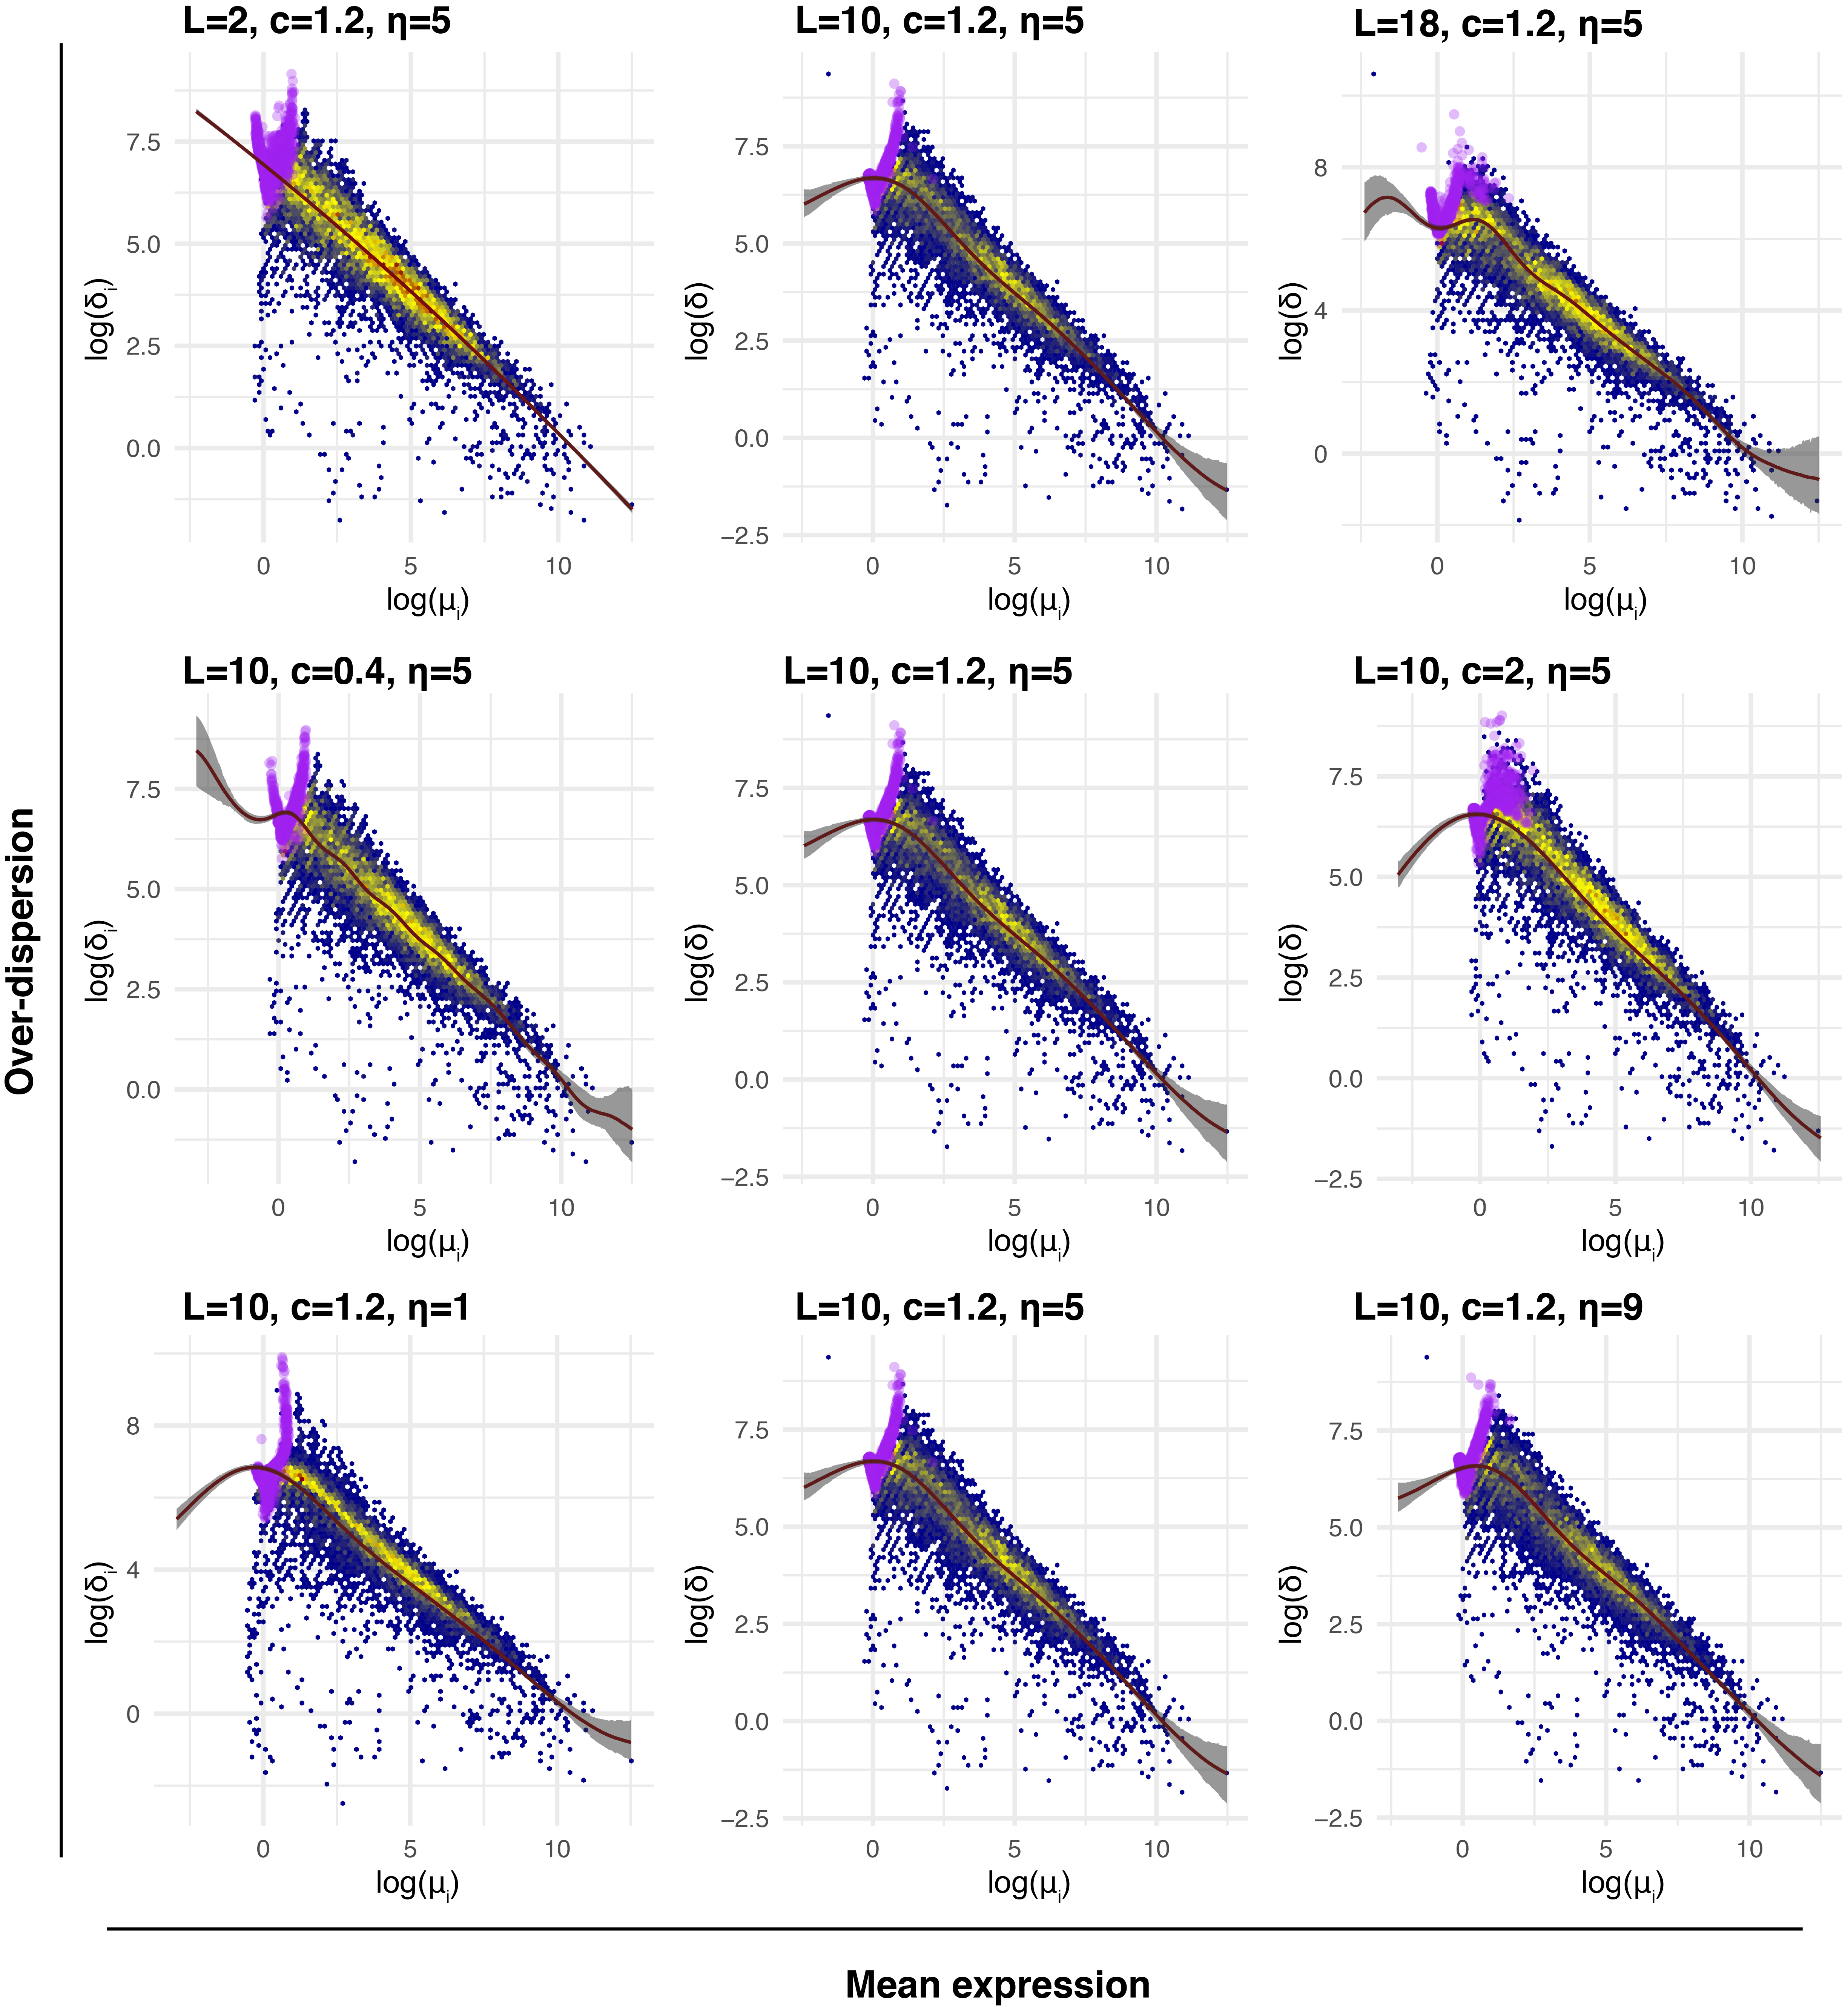
\includegraphics[width=0.9\textwidth]{Fig_4.png}
\caption[Characterisation of isolated CD4\plus{} T cells]{\textbf{Characterisation of isolated CD4\plus{} T cells (Full legend on next page).}}
\label{fig1:characterization}
\end{figure}

\newpage
\captionsetup[figure]{list=no}
\addtocounter{figure}{-1}   
\captionof{figure}{\textbf{Characterisation of isolated CD4\plus{} T cells (continued).}\\
\textbf{(A)} \emph{Cyclone} \citep{Scialdone2015} was used to classify individual naive and activated CD4\plus{} T cells into the cell cycle phases G1, G2/M and S, \textbf{(B)} \emph{TraCeR} \citep{Stubbington2015} constructed T cell receptor sequences from scRNA-Seq data to analyze clonal diversity in naive and activated CD4\plus{} T cells, \textbf{(C)} Cell sizes were estimated for naive and activated CD4\plus{} T cells in young and old B6 animals measured by FSC using flow cytometry, \textbf{(D)-(E)} CD4\plus{} T cells were purified from spleens of young (D) and old (E) B6 animals and stained with antibodies against CD4, CD62L, CD44, CD69, IL2R\textalpha{} (CD25), IL7R (CD127), and KLRG1 as well as viability dye. FACS plots shown are gated on single live cells (top left panel) and single live CD4\plus{} T cells (other panels), and percentages shown relate to total of gated cells, \textbf{(F)-(G)} Naive CD4\plus{} T cells were purified from spleens of five young (F) or two aged (G) B6 mice, and were either directly assayed or activated with plate-bound antibody against CD3\textepsilon{} and CD28 for 3 hours. Cells were stained with antibodies against CD4, CD69, and viability dye. Representative histograms for naive (red) and activated (blue) cells are shown, \textbf{(H)} Characterisation of possible differentiation processes leading to Th1, Th2, Th17, \gls{Treg} and Tfh cell lineages. For each lineage the major regulatory transcription factor (upper row) and an effector cytokine (lower row) is shown. Differential expression testing was performed between activated and naive cells from young B6 animals (left panel) and between activated and naive cells from old B6 animals (right panel). Upward arrow: up-regulation of expression (\gls{log2FC} in $\mu_i$ > 2, EFDR = 5\%) after activation, Downward arrow: down-regulation of expression (log2FC in $\mu_i$ > 2, EFDR = 5\%) after activation, \textbf{(I)} Heatmap showing T cell exhaustion (\textit{Pdcd1}, \textit{Lag3}, \textit{Havcr2}, \textit{Ctla4}) and TCR activation markers (\textit{Cd5}). Differential expression testing was performed in naive cells between young and old B6 animals (left panel) and in activated cells between young and old B6 animals (right panel). Upward arrow: up-regulation of expression (log2FC in $\mu_i$ > 2, EFDR = 5\%) during ageing, \textbf{(J)} Th1 lineage marker (\textit{Tbx21}, \textit{Ifng}) expression was compared between B6 and CAST in following conditions: naive cells from young animals (upper left panel), naive cells from old animals (lower left panel), activated cells from young animals (upper right panel), activated cells from old animals (lower right panel). \#: statistically significant differential expression (log2FC in $\mu_i$ > 2, EFDR = 5\%), \textbf{(K)} Th2 lineage marker (\textit{Gata3}, \textit{Il4}) expression was compared between B6 and CAST in the following conditions: naive cells from young animals (upper left panel), naive cells from old animals (lower left panel), activated cells from young animals (upper right panel), activated cells from old animals (lower right panel). From \citep{Martinez-jimenez2017}. Reprinted with permission from AAAS.\\}
\captionsetup[figure]{list=yes}

After the above analyses and the experimental characterisation, a total of 1514 high-quality CD4\plus{} T cell transcriptomes from young and old animals were analysed across all conditions (unstimulated and activated; naive, FACS-purified naive, FACS-purified EM) and species (B6 and CAST). An overview of all high-quality transcriptomes can be seen in \textbf{Fig.~\ref{fig1:all_cells}}. We detect that unstimulated and stimulated cells group together \textbf{(Fig.~\ref{fig1:all_cells}A)} while separation is also noticeable between species \textbf{(Fig.~\ref{fig1:all_cells}B)} and experimental methods \textbf{(Fig.~\ref{fig1:all_cells}C)}. As discussed below, cells from young and old animals do not separate when visualising the cells in form of a tSNE  \textbf{(Fig. \ref{fig1:all_cells}C)}. 

\newpage

\begin{figure}[!hb]
\centering
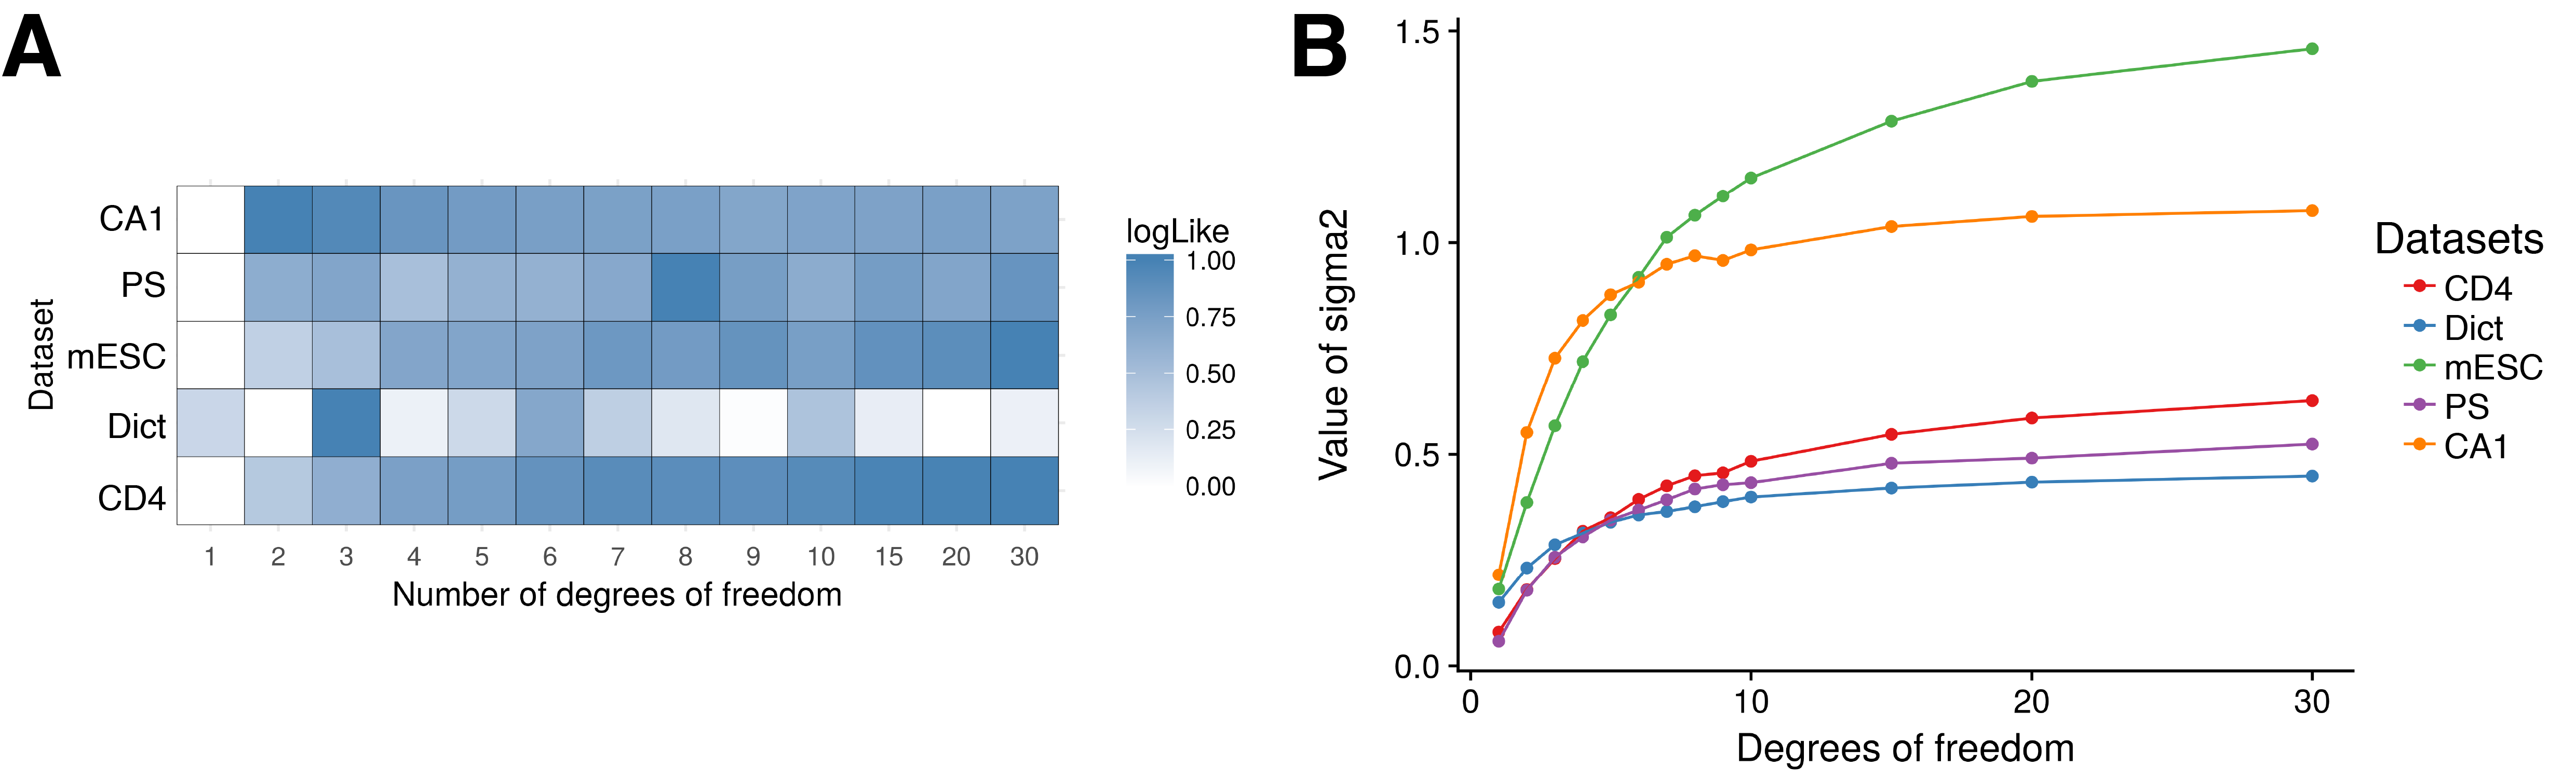
\includegraphics[width=\textwidth]{Fig_5.png}
\caption[Visualisation of all isolated CD4\plus{} T cells]{\textbf{Visualisation of all isolated CD4\plus{} T cells.}\\
tSNE dimensionality reduction of 1514 CD4\plus{} T cells isolated from young and old mice of two related species. Cells were labelled based on \textbf{(A)} their activation state, \textbf{(B)} the mouse species, \textbf{(C)} experimental isolation approach and \textbf{(D)} age.}
\label{fig1:all_cells}
\end{figure}

\newpage

\section{Species-specific gene expression in naive CD4\plus{} T cells}

To characterise the variation observed in \textbf{Fig.~\ref{fig1:all_cells}}, we firstly dissected differences in gene expression between the two different mouse species using naive CD4\plus{} T cells. We also assessed whether possible differences that are detected between the two species are driven by differences in the assembly of the genome reference.

\subsection{Avoiding gene counting biases due to incorrect alignment}

We used BASiCS \citep{Vallejos2016} to detect differentially expressed genes as described in \textbf{Section \ref{sec1:computational}}. In scRNA-Seq, technical noise is highest for lowly expressed genes \citep{Brennecke2013} and we therefore excluded genes that had an average posterior mean expression < 50 in each population. Subsequently, we applied the differential expression test developed within BASiCS, using a threshold of log2FC in $\mu_i$ > 2 with the EFDR controlled to 5\%. We observed that 15\% of expressed genes were differentially transcribed between CD4\plus{} T cells of the two mouse species \textbf{(Fig. \ref{fig1:spec_spec_mapping}A)}. 

\begin{figure}[!hb]
\centering
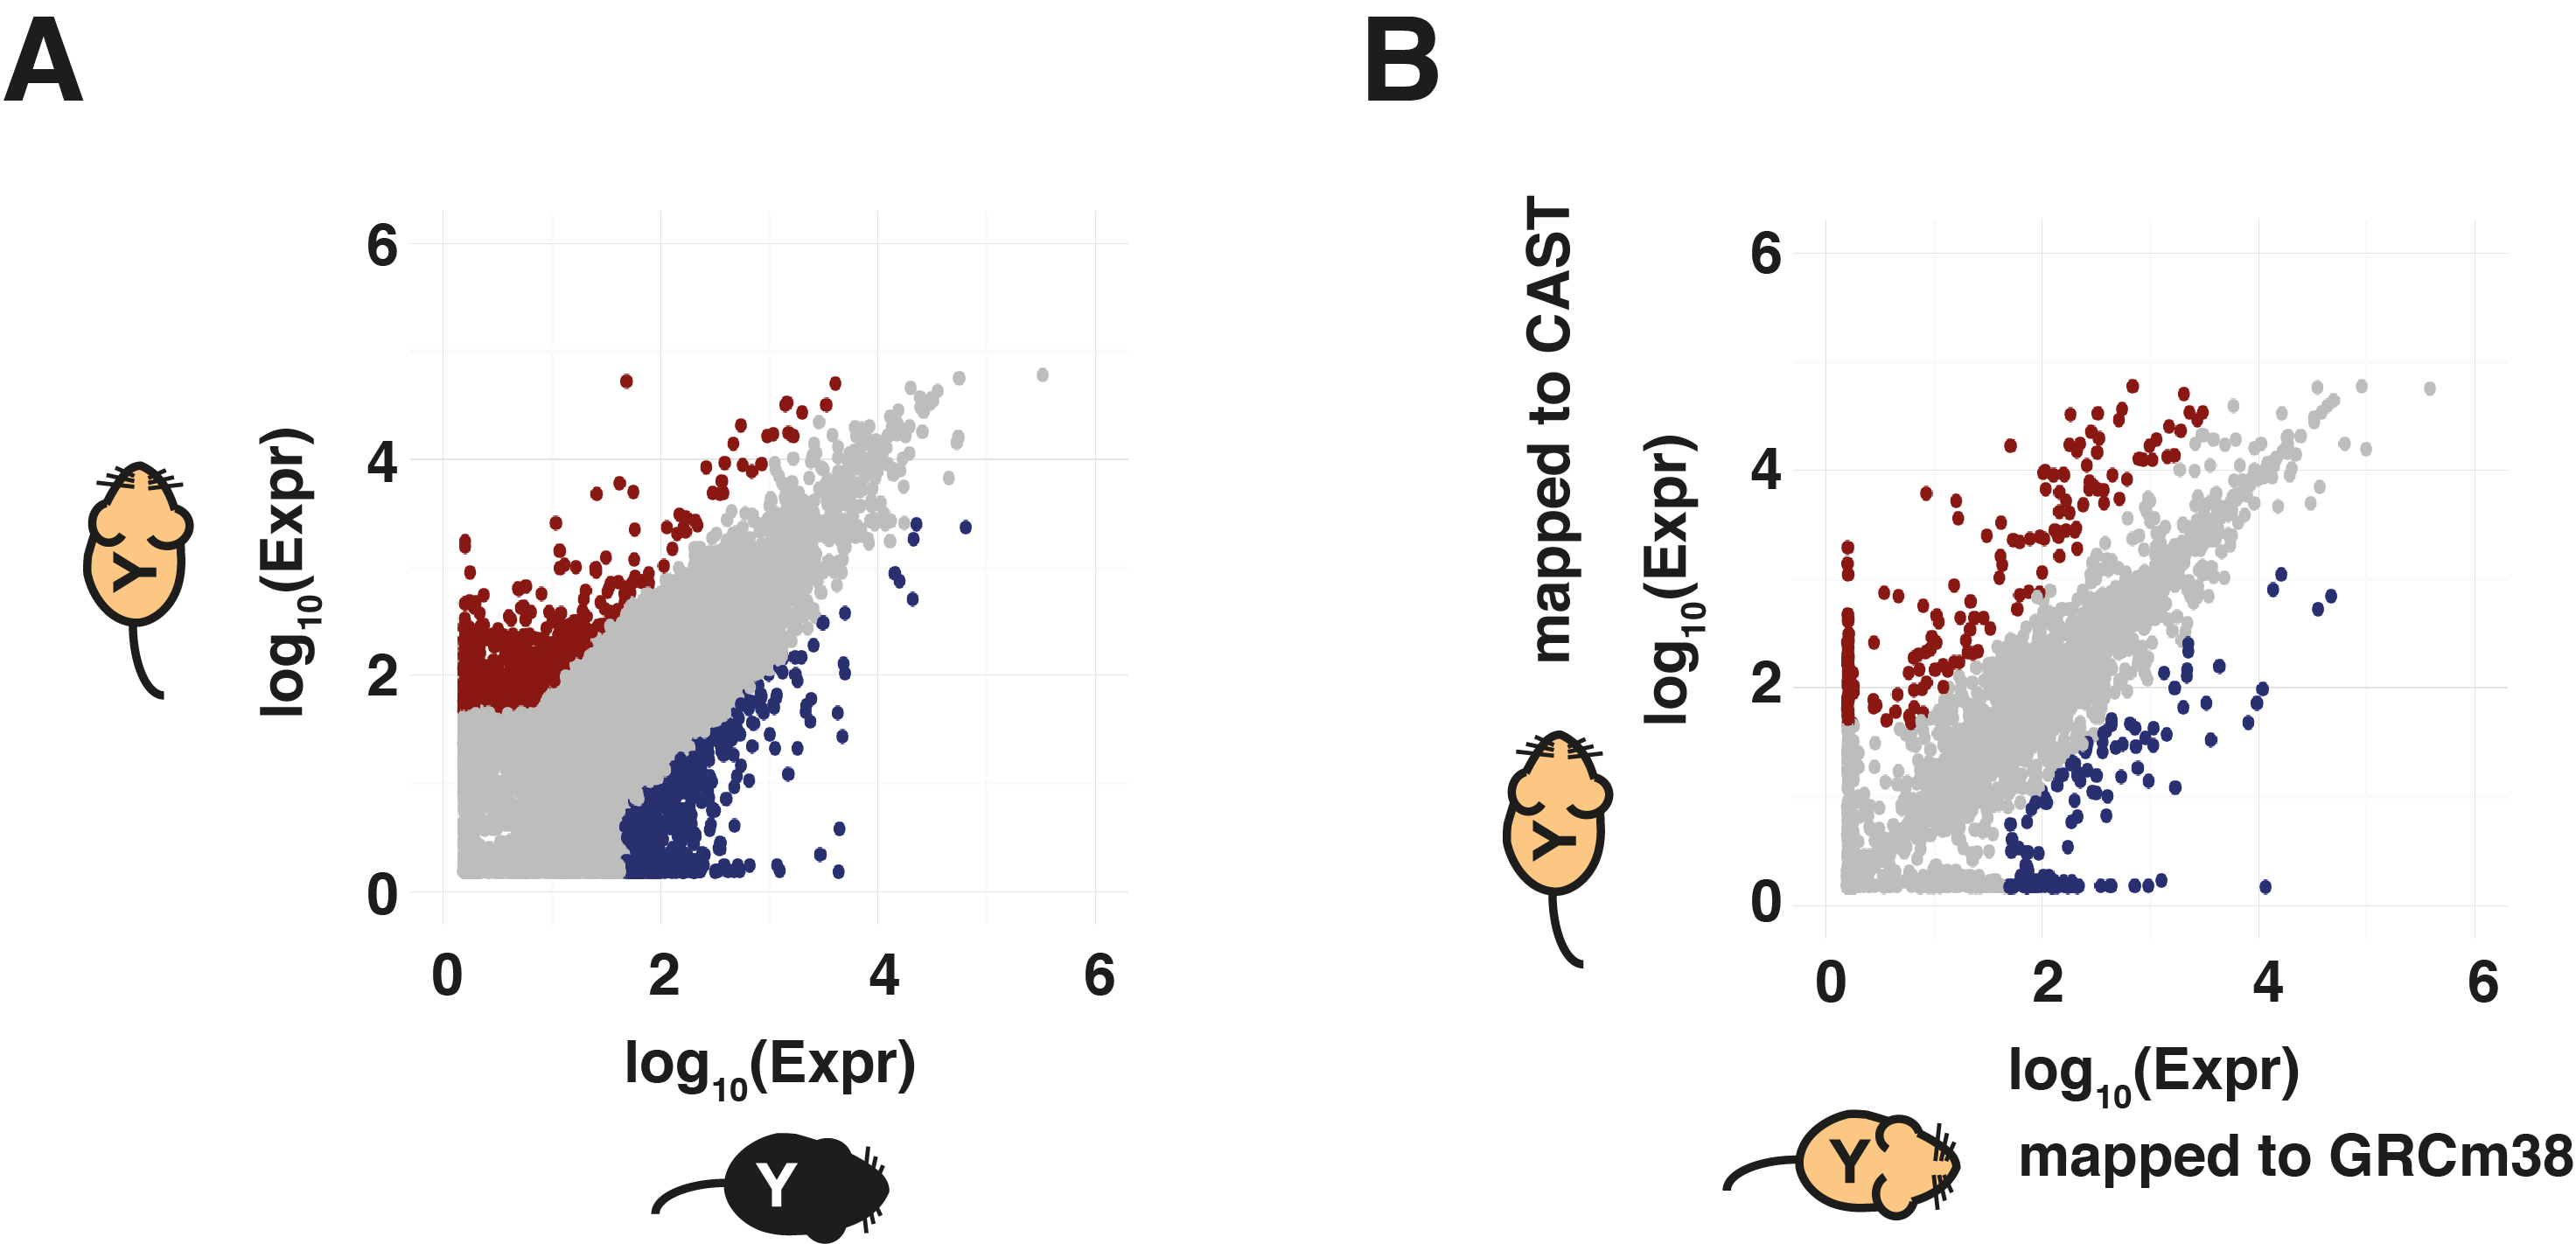
\includegraphics[width=0.8\textwidth]{Fig_7.png}
\caption[Cross-mapping correction between divergent mouse species]{\textbf{Cross-mapping correction between divergent mouse species.}\\
\textbf{(A)} Species-specific gene expression in B6 (blue) or CAST (red). Average gene expression using posterior estimation, threshold of means > 50, log2FC in $\mu_i$ > 2, EFDR = 5\%, \textbf{(B)} Mean, normalised transcript counts of mapped reads from CAST cells (young, naive) using the GRCm38 genome (x-axis) or the CAST genome (y-axis) as reference. Differentially mapped genes were removed from downstream analysis. Average gene expression using posterior estimation, threshold of means > 50, log2FC in $\mu_i$ > 2, EFDR = 5\%.
}
\label{fig1:spec_spec_mapping}
\end{figure}

To rule out the possibility that these differences are driven by potential artefacts in the new \textit{Mus musculus castaneus} genome assembly, we also mapped reads from young CAST samples to the GRCm38 genome. To estimate which differentially expressed genes may arise due to errors in the new CAST genome assembly, we performed the same differential expression analysis on CAST samples by mapping these libraries onto both GRCm38 and CAST. Roughly 5\% of all tested genes are detected as differentially expressed even though the samples being compared are identical and only mapped to different genomes \textbf{(Fig. \ref{fig1:spec_spec_mapping}B)}. Comparing this set of genes to the set of species-specific genes, we find that they make up 10\% of differentially expressed genes between the two species. We performed a similar analysis for B6 samples. This approach allowed us to remove genes which show differences in expression from our analyses, which may be driven by the quality of the reference genome.

\subsection{Transcriptional dynamics of species-specific genes}
\label{sec1:species-spec-dynamics}

Similar for \textbf{Fig.~\ref{fig1:all_cells}}, we found that CD4\plus{} T cells cluster by species when only profiling naive cells \textbf{(Fig.~\ref{fig1:species_specific}A)}. As described above, theses differences are driven by the roughly 15\% of differentially expressed genes. To assess the functional role of the species-specific genes that are not due to biases in read alignment, we qualitatively and quantitatively compared their expression across individual cells in both species. Firstly, species-specific genes were only expressed in subsets of the full population of naive CD4\plus{} T cells \textbf{(Fig.~\ref{fig1:species_specific}B)}. Furthermore, we used DAVID \citep{Dennis2003} to test for \gls{GO} enrichment in differentially expressed gene sets. In line with genes being only sporadically expressed across the full population of cells, we did not detect functional enrichment in either B6 or CAST specific genes \textbf{(Fig.~\ref{fig1:species_specific}C)}. Profiling individual cells using scRNA-Seq allows us to detect different patterns of expression for species-specific genes. Within the set of species-specifically expressed genes, we detect some that display low variability and some with high variability \textbf{(Fig.~\ref{fig1:species_specific}D)}. More quantitatively, when profiling expression variability, we detect species-specifically transcribed genes to be generally more variable on a cell-to-cell basis than genes expressed in both species \textbf{(Fig. \ref{fig1:species_specific}E)}. These findings hint that the detected divergence in genes expression might be caused by neutral drift without functional support of the species-specific genes. We therefore argue that profiling transcriptional variability in a homogeneous population of cells is a redundant measure for cell-population function such as cell response to stimuli.

\newpage

\begin{figure}[!h]
\centering
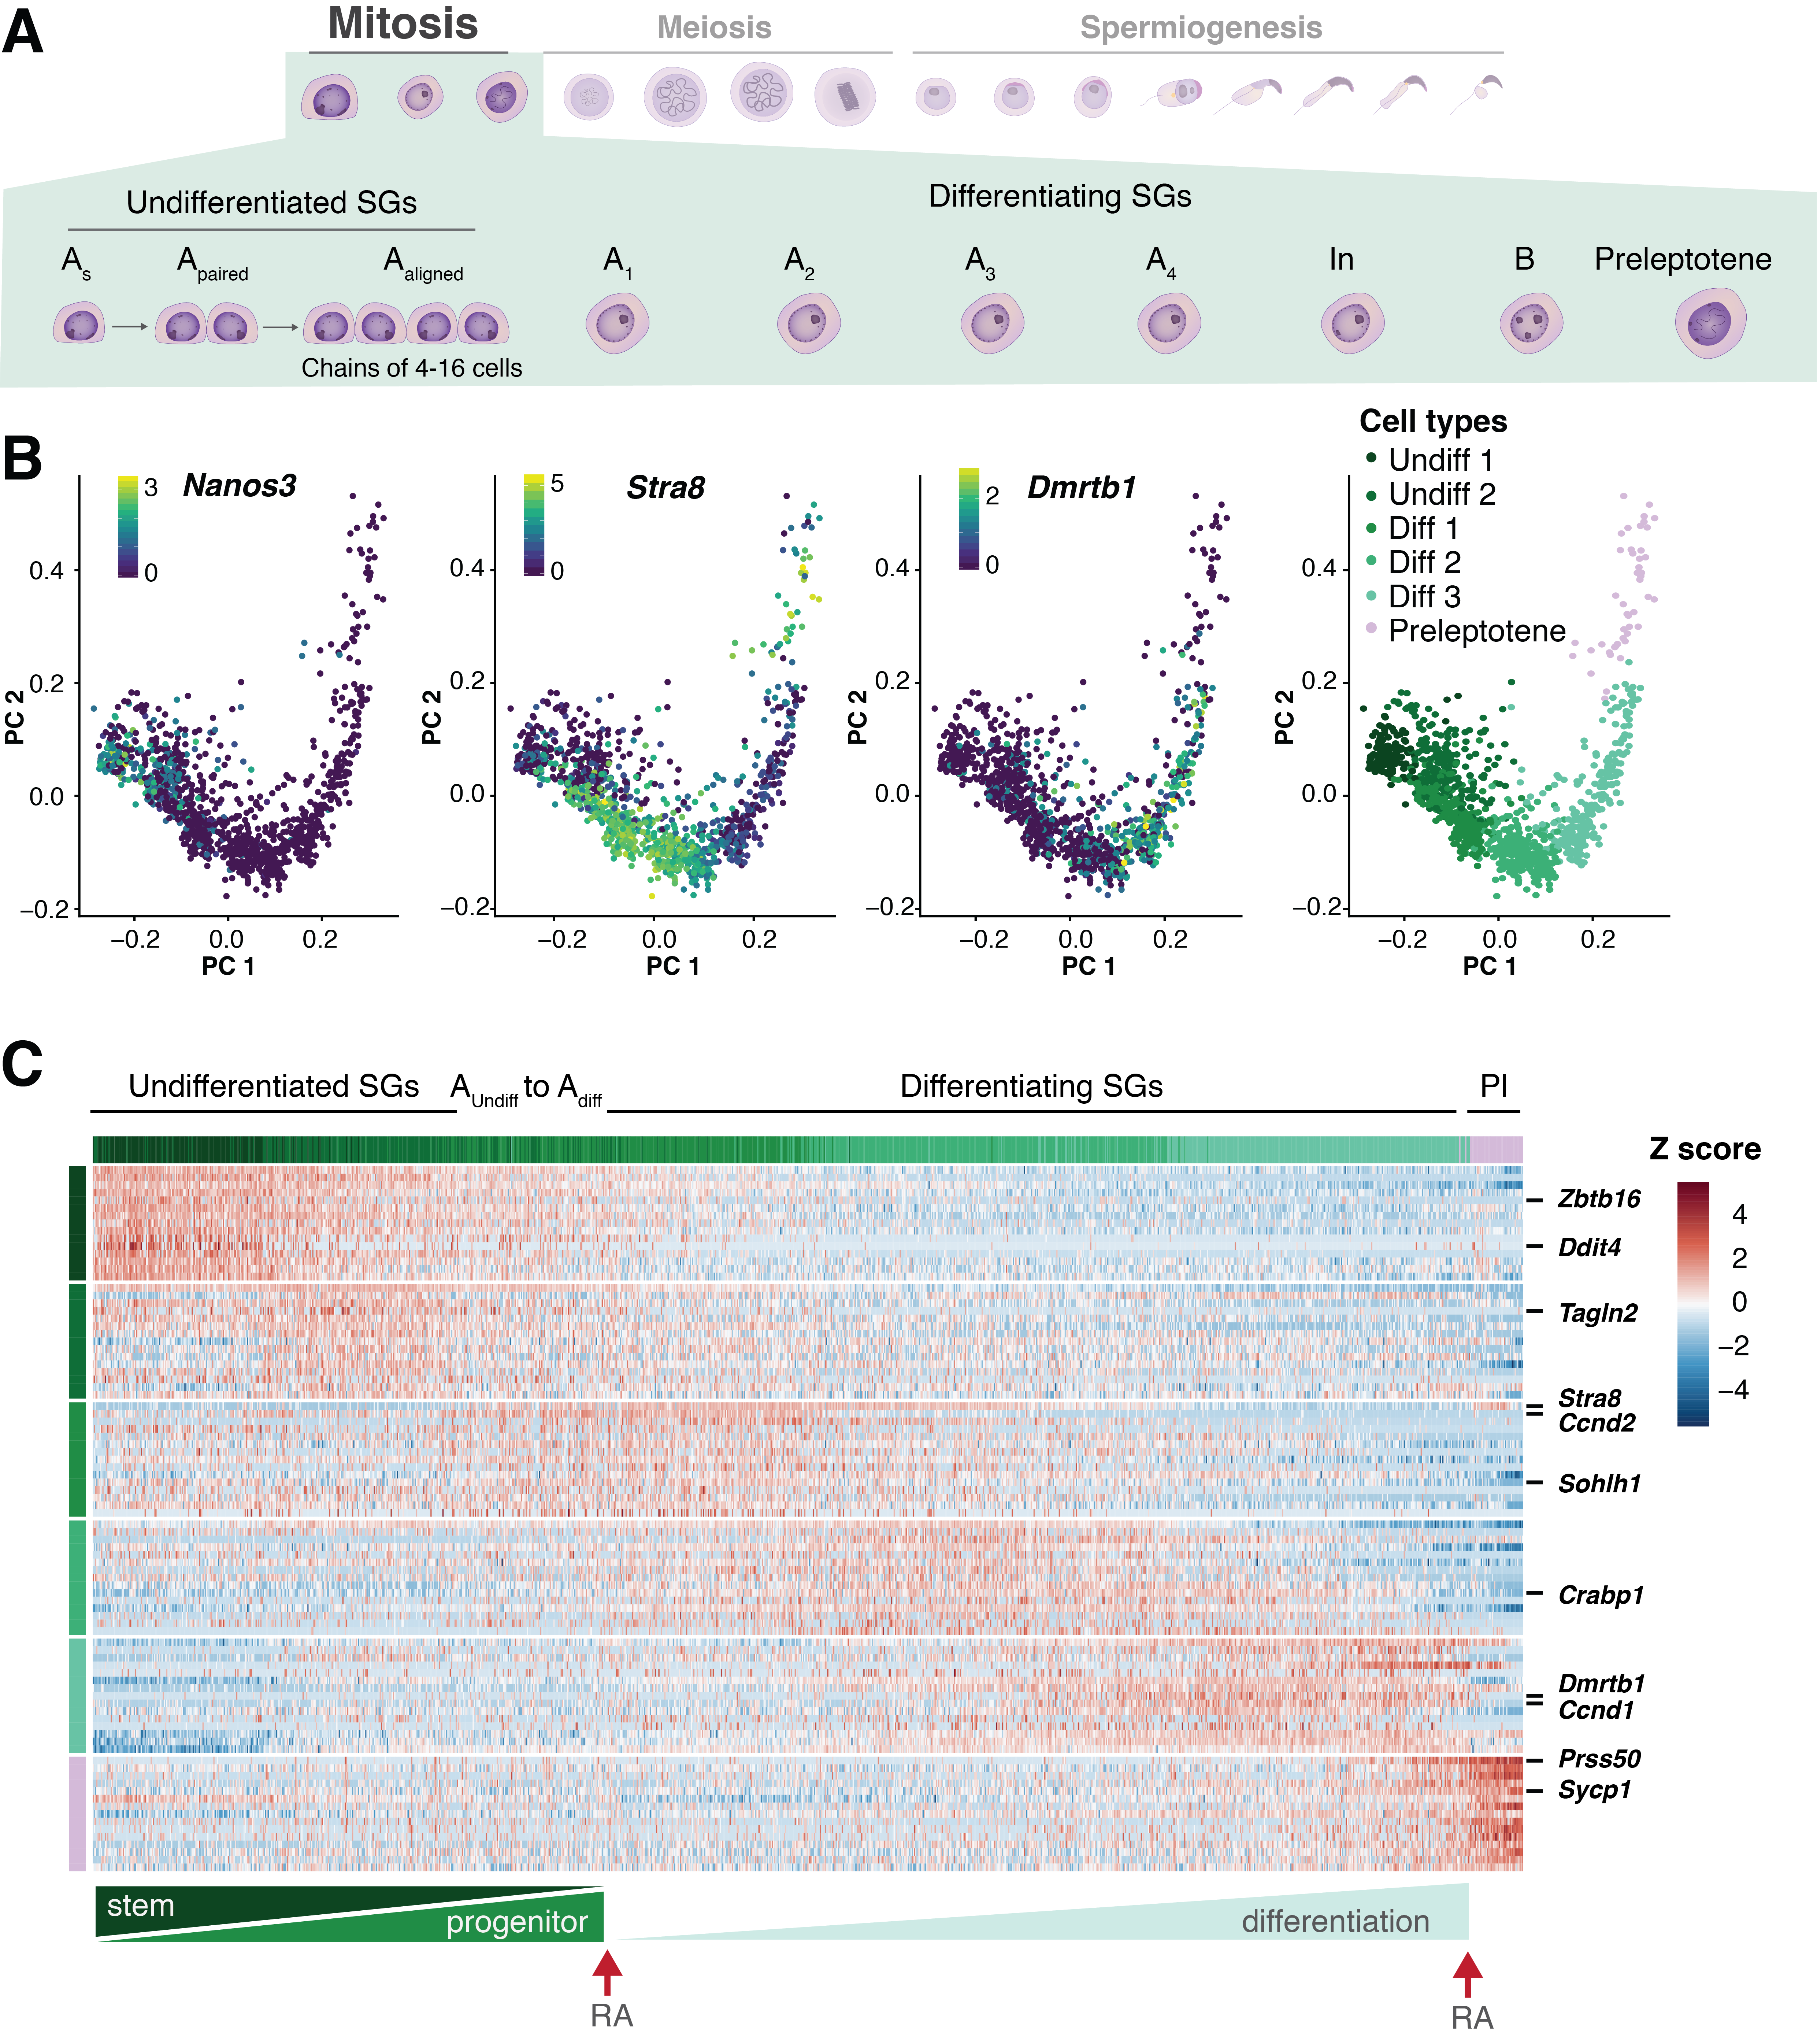
\includegraphics[width=0.9\textwidth]{Fig_6.png}
\caption[Species-specific gene expression in naive CD4\plus{} T cells]{\textbf{Species-specific gene expression in naive CD4\plus{} T cells.}\\
\textbf{(A)} tSNE dimensionality reduction of scRNA-Seq data reveals species-specific clustering of naive CD4\plus{} T cells from young animals, \textbf{(B)} Representative heatmap of 30 genes and 30 cells randomly selected from all species-specifically transcribed genes from young animals shows typical species-specific variations \textbf{(C)}  GO analysis of species-specific genes. Bonferroni corrected p-values (adjusted p-values) were used to visualise GO enrichment. The statistical significance threshold was set to adjusted p-value = 0.1 (red line), \textbf{(D)} Cell-to-cell variability in gene expression levels. Violin plots show distribution of single-cell expression of selected species-specifically transcribed genes (in grey background), ranked from lowest (top) to highest variability (bottom), \textbf{(E)} $\log_{10}$-transformed variability estimates of species-specific genes were compared to variability estimates of all genes expressed in B6 (left) and CAST (right). Mann-Whitney-Wilcoxon test; ***: p<10$^{-10}$}.
\label{fig1:species_specific}
\end{figure}

\newpage


\section{Expression dynamics during CD4\plus{} T cell activation}
\label{sec1:activation}

Functional CD4\plus{} T cell transcriptional responses start with an early, targeted activation of translational machinery and cytokine networks, followed by large-scale transcriptional changes associated with lineage commitment \citep{Shay2013, Asmal2003}. To characterise the immediate early activation program, we stimulated naive CD4\plus{} T cells of B6 animals for three hours with plate-bound anti-CD3\textepsilon{}/anti-CD28 antibodies, thus inducing a strong and uniform activation mimicking initial contact with an antigen-presenting cell. Importantly, we did not use additional cytokines to commit the naive CD4\plus{} T cells to specific helper cell lineages \citep{Zhu2010}. This was confirmed empirically by the analysis presented in \textbf{Section \ref{sec1:characterization}}. 

\subsection{Mean expression changes during immune activation}

By visualising the dimensionality reduced transcriptional profiles of naive and activated CD4\plus{} T cells, we qualitatively observe strong transcriptional changes during immune activation \textbf{(Fig.~\ref{fig1:immune_activation}A)}. Differential mean expression testing identifies thousands of genes as differentially expressed in CD4\plus{} T cells upon activation (2063 genes, log2FC in $\mu_i$ > 2, EFDR = 5\%) \textbf{(Fig.~\ref{fig1:immune_activation}B)}. We sought to investigate the behaviour of up- and down-regulated genes across the population of naive or activated cells. Initially, we calculated, for each gene, the percentage of cells in which it was expressed (> 0 transcript counts). Genes whose expression is down-regulated after activation are expressed in a median of 18\% naive CD4\plus{} T cells isolated from B6, while genes that are up-regulated are expressed in a median of 36\% activated cells. Before activation, up-regulated genes are only expressed in a median of 5\% naive cells while after activation, down-regulated genes are expressed in a median of 4\% activated cells \textbf{(Fig.~\ref{fig1:immune_activation}C)}. This analysis suggests that the immune response genes are similarly up-regulated across all cells, while genes that are down-regulated upon immune activation are more sporadically expressed in naive cells. \\

Furthermore, we performed GO analysis on genes either up- or down-regulated \textbf{(Fig.~\ref{fig1:immune_activation}D)}. Among the genes down-regulated are components of the intra-cellular signalling network while genes that are up-regulated are mostly part of the translation machinery \citep{Bjur2013}. Furthermore, the transcriptional switch driven by TCR engagement and co-stimulation included classic markers of activation, including (\textit{\gls{Il2ra}}, \textbf{Fig.~\ref{fig1:immune_activation}E}) and \textit{\gls{Ccl4}} \citep{Asmal2003}. In contrast, we observed the coordinated suppression of \textit{Sell} (\textit{Cd62l}, \textbf{Fig.~\ref{fig1:immune_activation}F}), as expected after activation \citep{Park2005}.

\newpage

\begin{figure}[!ht]
\centering
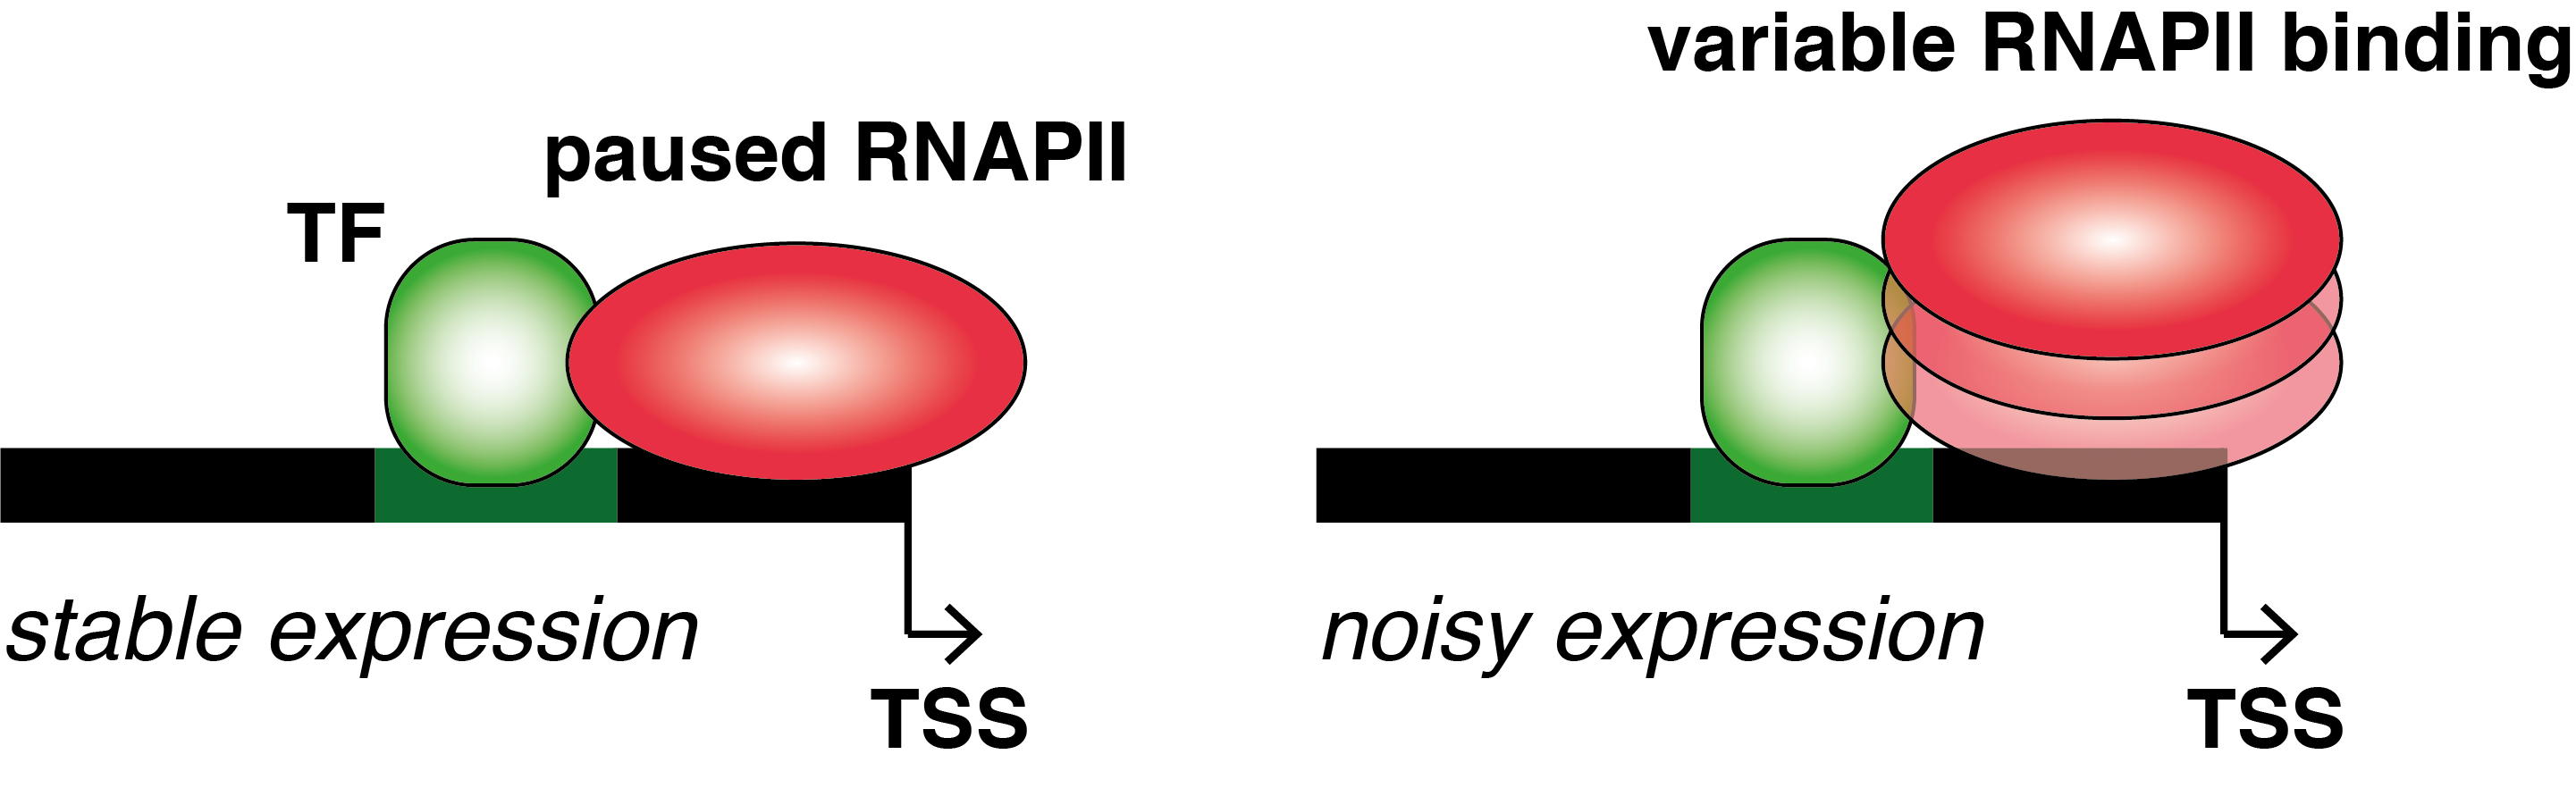
\includegraphics[width=0.9\textwidth]{Fig_8.png}
\caption[Mean expression dynamics upon CD4\plus{} T cell activation]{\textbf{Mean expression dynamics upon CD4\plus{} T cell activation.}\\
\textbf{(A)} Activation of CD4\plus{} T cells from young B6 mice induces large-scale transcriptional changes which is visualised using tSNE dimensionality reduction, \textbf{(B)} Genes up-regulated (red) and down-regulated (blue) by immune stimulation in young B6 mice. Non-differentially expressed genes shown in black. Average gene expression using posterior estimation, threshold of means > 50, log2FC in $\mu_i$ > 2, EFDR = 5\%, \textbf{(C)} Fractions of cells in which down- or up-regulated genes are expressed (600 genes were randomly selected, histograms with 50 bins, median value is indicated). Upper panels: fraction of naive (left) and activated (right) cells in which down-regulated genes are expressed. Lower panels: fraction of naive (left) and activated (right) cells in which up-regulated genes are expressed, \textbf{(D)} Bar plots of functional gene categories enriched in up- and down-regulated genes during activation of CD4\plus{} T cells in B6 (Bonferroni multiple testing corrected p-values, red line marking 0.1), \textbf{(E)} Example genes that represent transcriptional changes upon activation of CD4\plus{} T cells: \textit{Il2ra} (CD25) is highly and consistently up-regulated after stimulation, \textbf{(F)} \textit{Cd62l} (\textit{Sell}) is more stochastically expressed in naive CD4\plus{} T cells, and is down-regulated upon activation.
}
\label{fig1:immune_activation}
\end{figure}

\newpage

\subsection{Changes of expression variability during immune activation}

We next profiled changes in expression variability upon immune activation. Due to the strong confounding effect observed between mean expression and variability estimates, we only profiled genes that show no changes in mean expression between the naive and activated state (see \textbf{Section \ref{sec1:computational}}, indicated as black dots in \textbf{Fig. \ref{fig1:immune_variability}A}, log2FC in $\mu_i$ = 0, EFDR = 5\%). When comparing posterior medians of the over-dispersion parameter $\delta_i$ for genes that remain stable in mean expression, we observed a significant reduction in cell-to-cell transcriptional variability (Mann-Whitney-Wilcoxon test, p<10$^{-10}$) \textbf{(Fig.~\ref{fig1:immune_variability}B)}. For example, the \textit{\gls{Eif1}}, show a marked decrease in cell-to-cell transcriptional variability, consistent with increased regulatory coordination \textbf{(Fig. \ref{fig1:immune_variability}C)}.\\

We next investigated whether genes that are more variably expressed in the naive than the activated condition showed coordinated patterns of expression, which are potentially associated with cryptic substructure. For this, we identified genes with statistically higher expression variability in the naive population compared to activated cells (log2FC in $\delta_i$ > 0.4, EFDR = 5\%, no change in mean expression). Genes with high variability and high pairwise correlation (Spearman’s $\rho$ > 0.8) in the naive population can be used to identify possible sub-populations of CD4\plus{} T cells. A hierarchical clustering analysis did not show any signs of such substructure \textbf{(Fig. \ref{fig1:immune_variability}D)}. This analysis therefore indicates that the collapse in variability is cause by a genuine shift from stochastic to regulated expression between two homogeneous populations of cells.\\

Finally, it has been observed that covariance between cells due to unobserved factors such as the cell cycle can mask potentially interesting biological signals \citep{Stegle2015, Buettner2015}. In our dataset, ribosomal biogenesis is the strongest mediator of CD4\plus{} T cell function upon activation which is strongly and homogeneously expressed across all cells \textbf{(Fig.~\ref{fig1:immune_activation}D and Fig.~\ref{fig1:immune_variability}C)}. We therefore regressed out this factor using a latent variable model (scLVM, \citep{Buettner2015}) to uncover underlying variance in activated CD4\plus{} T cells. Importantly, performing PCA on the uncorrected and corrected counts after regression did not reveal concealed cellular processes \textbf{(Fig.~\ref{fig1:immune_variability}E)}.\\

\newpage


\begin{figure}[!ht]
\centering
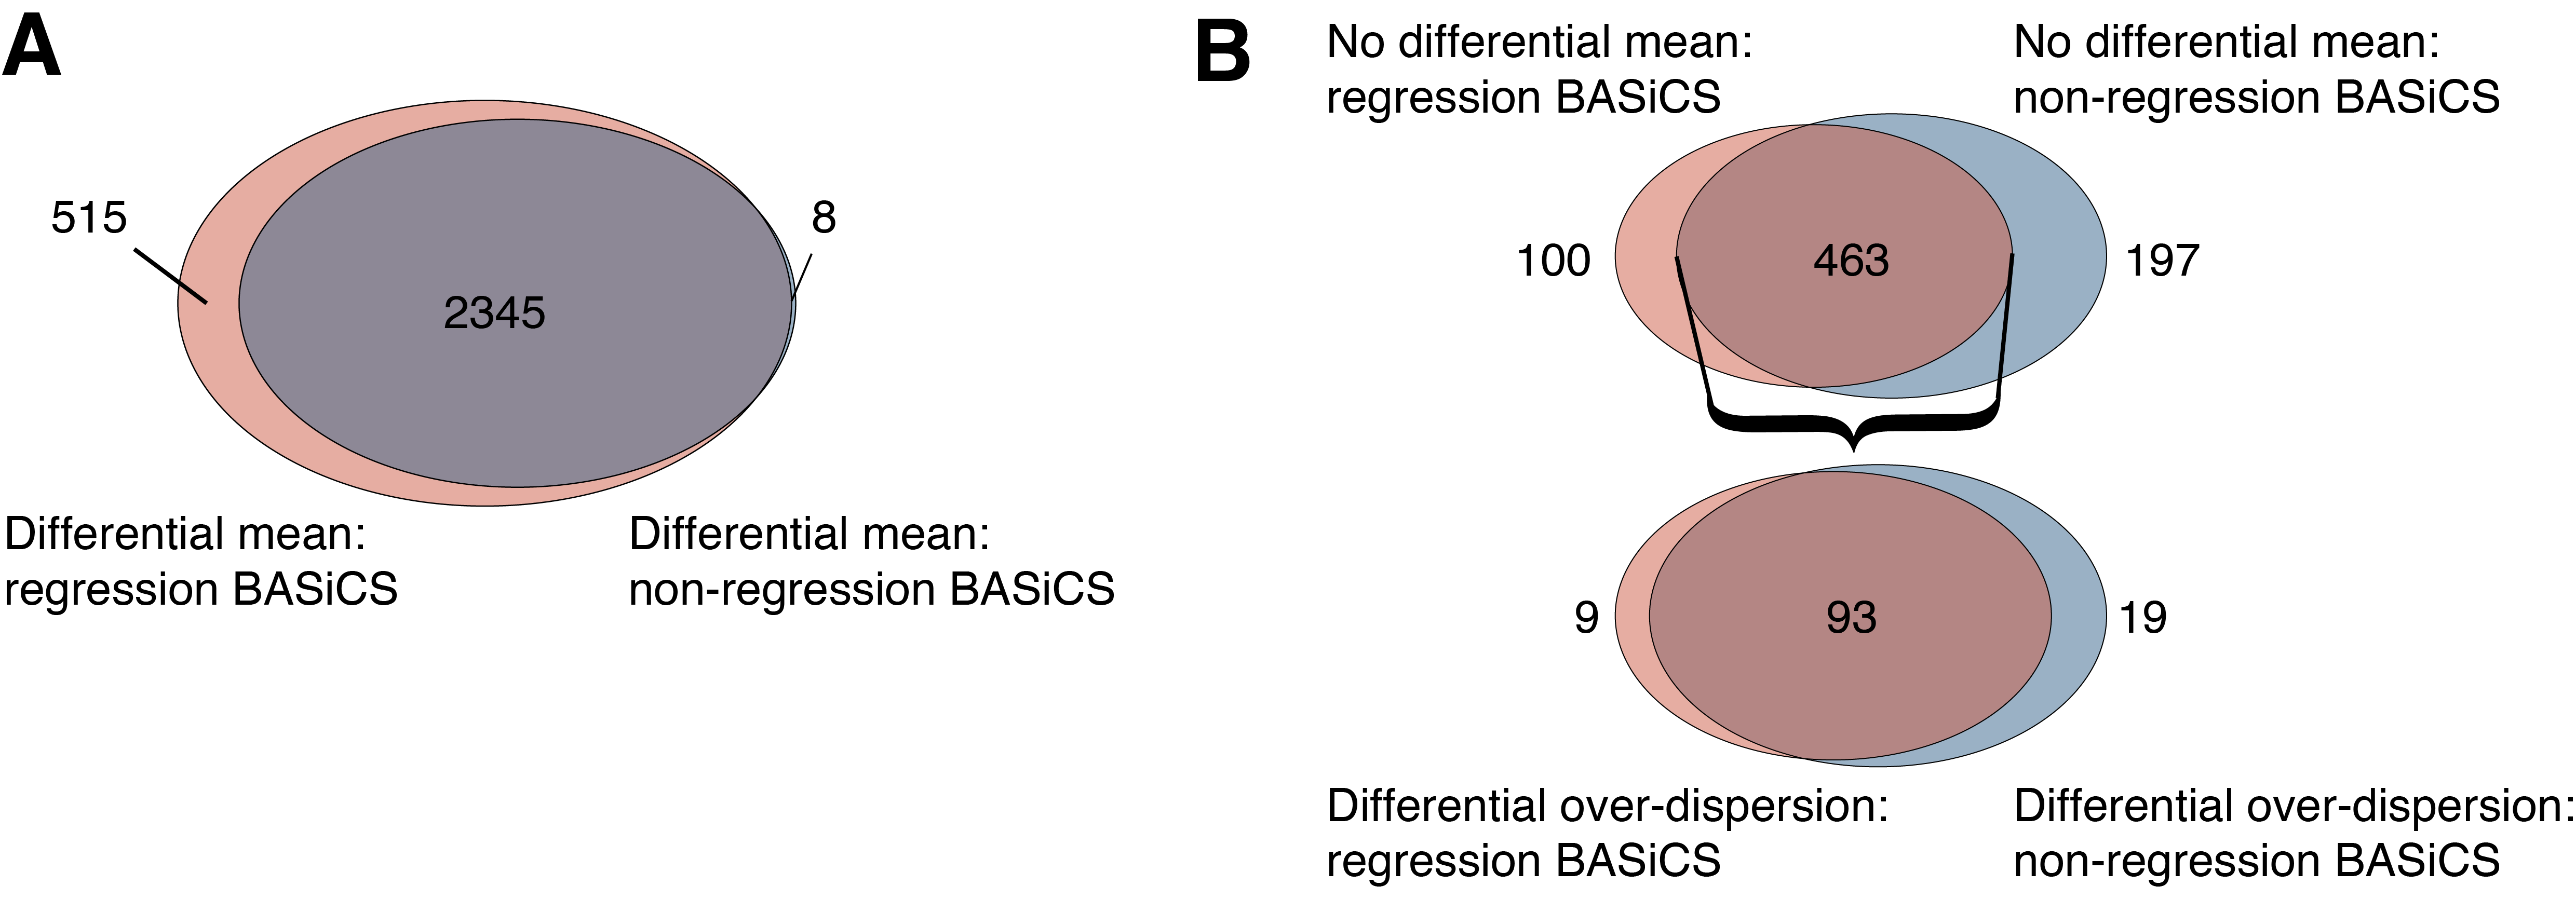
\includegraphics[width=\textwidth]{Fig_9.png}
\caption[Changes in transcriptional variability upon immune activation]{\textbf{Changes in transcriptional variability upon immune activation.}\\
\textbf{(A)} Genes up-regulated (red) and down-regulated (blue) by immune stimulation in young B6 mice (log2FC in $\mu_i$ > 2, EFDR = 5\%). Non-differentially expressed genes shown in black (log2FC in $\mu_i$ = 0, EFDR = 5\%). Average gene expression using posterior estimation, threshold of means > 50, \textbf{(B)} Genes with no overall gene expression differences during activation (black dots in (A)) show decreased cell-to-cell variability in transcription (Mann-Whitney-Wilcoxon test, ***: p<10$^{-10}$), \textbf{(C)} \textit{Eif1} is expressed in most cells in both conditions at similar levels, but shifts from stochastic to regulated expression, \textbf{(D)} To detect possible sub-populations in naive or activated CD4\plus{} T cells, differentially variable genes (log2FC in $\delta_i$ > 0.4, EFDR = 5\%) in naive cells with high gene-to-gene correlation (Spearman’s $\rho$ > 0.8) were used for hierarchical cluster analysis, \textbf{(E)} Upper panel: PCA of normalised counts of activated CD4\plus{} T cells from young B6 animals. Lower panel: PCA of activated CD4\plus{} T cells of young B6 animals after removing differences in the translation program as a confounding factor.}
\label{fig1:immune_variability}
\end{figure}

\newpage


\subsection{Response-related transcriptional dynamics in CAST}

As described above, activation of CD4\plus{} T cells drives a transcriptional switch that alters the global expression profile from a stochastic to a tightly regulated state. To test whether these transcriptional dynamics are evolutionarily conserved, we performed the same analysis for CD4\plus{} T cells extracted from CAST. Similar to cells isolated from young B6, we detect (i) clustering based on activation state \textbf{(Fig. \ref{fig1:immune_activation_CAST}A)}, (ii)  thousands of genes being differentially expressed \textbf{(Fig. \ref{fig1:immune_activation_CAST}B)}, (iii) a decrease in expression variability after immune activation for genes that are stable in mean expression \textbf{(Fig. \ref{fig1:immune_activation_CAST}C)} and (iv) the expression of up-regulated genes in a higher number of activated cells than down-regulated genes in naive cells \textbf{(Fig. \ref{fig1:immune_activation_CAST}D)}.

\begin{figure}[!ht]
\centering
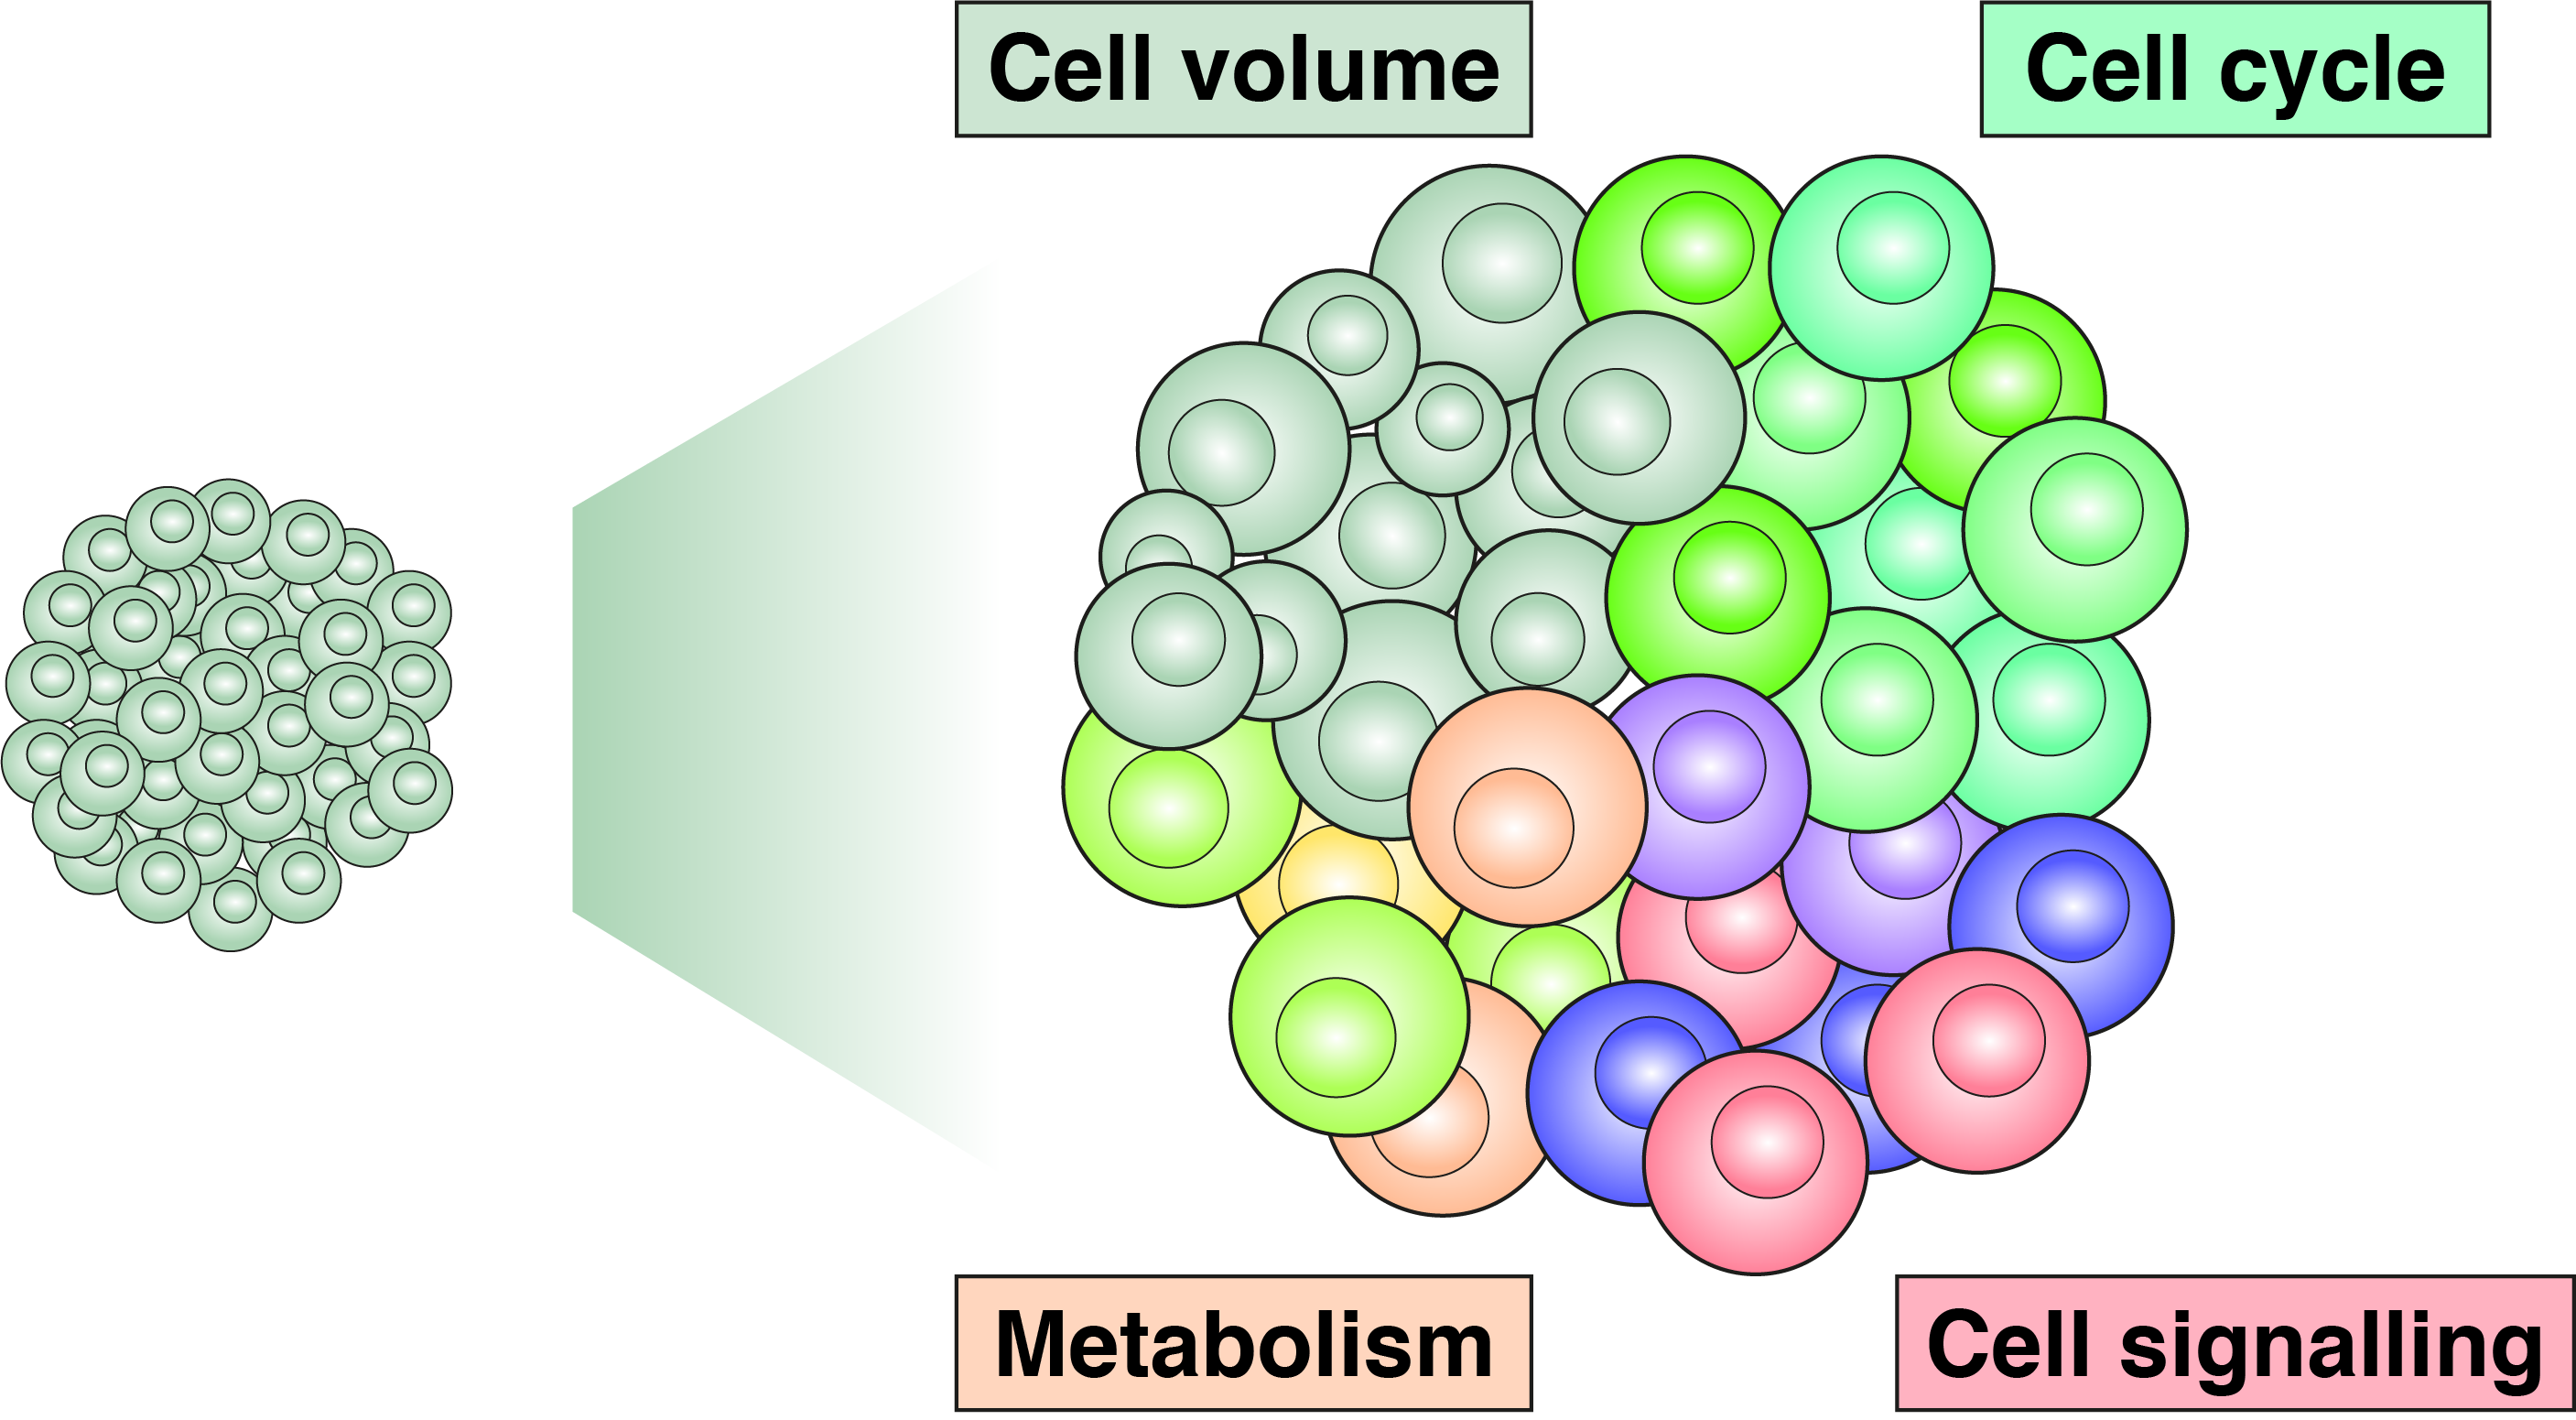
\includegraphics[width=0.65\textwidth]{Fig_10.png}
\caption[Immune activation dynamics in young CAST animals]{\textbf{Immune activation dynamics in young CAST animals.}\\
\textbf{(A)} Activation of CD4\plus{} T cells from young CAST mice in anti-CD3\textepsilon{}/CD28 coated plates induces large-scale transcriptional changes, visualised using tSNE dimensionality reduction, \textbf{(B)} Genes up-regulated (red) and down-regulated (blue) by immune stimulation in young CAST mice (log2FC in $\mu_i$ > 2, EFDR = 5\%). Non-differentially expressed genes used in (C) are shown in black (log2FC in $\mu_i$ = 2, EFDR = 5\%). Average gene expression using posterior estimation, threshold of means > 5, \textbf{(C)} Genes with no overall gene expression differences during activation show decreased cell-to-cell variability in transcription (Mann-Whitney-Wilcoxon test, ***: p<10$^{-10}$), \textbf{(D)} Up-regulated genes were expressed in a relatively large fraction of activated CD4\plus{} T cells after stimulation (median 25\%). Down-regulated genes were expressed in a smaller fraction of naive CD4\plus{} T cells (median 17\%). 600 genes of each condition were randomly selected. From \citep{Martinez-jimenez2017}. Reprinted with permission from AAAS.}
\label{fig1:immune_activation_CAST}
\end{figure}

\newpage

\section{Conservation of the core activation process}

As shown above, we detect similar activation patterns when comparing CD4\plus{} T cell activation between B6 and CAST. To further study the conservation of this immune response, we used the rapid divergence in gene expression between CD4\plus{} T cells from both species to refine the functional set of immune response genes activated upon immune stimulation \citep{Shay2013}. Conserved functionality is assumed when genes are similarly up-regulated upon activation in both species. We hypothesise that such targets would be both conserved between species and expressed in most cells, whereas the genes activated species-specifically would be less likely to be functional targets and more likely to be sporadically expressed.

\subsection{Detecting evolutionarily conserved response genes}

As described for B6 above, we stimulated naive CD4\plus{} T cells isolated from young CAST males using anti-CD3\textepsilon{}/anti-CD28 antibodies followed by scRNA-Seq. As expected, cells clustered based on their activation state and species of origin \textbf{(Fig.~\ref{fig1:shared_activation}A)}. To find genes that form the evolutionarily conserved, core activation program, we test for differential expression between the naive and activated state separately in B6 and CAST (log2FC in $\mu_i$ > 2, EFDR = 5\%). Genes that are up-regulated after activation similarly in B6 and CAST form the shared activation program. Up-regulated genes that are differentially expressed in activated cells between the two species (log2FC in $\mu_i$ > 2, EFDR = 5\%) represent the species-specific response genes. \\

We next ensured that the species-specific differences in transcriptional response are not caused by mapping artefacts between the different genome builds. For this, we quantified gene expression in activated CAST and B6 samples based on the CAST and GRCm38 genome as described above. Genes in the activated state that show differential mapping between the two genomes were excluded from the species-specific lists of response genes. After removing those, we find 1208 genes to be up-regulated across both species. Out of these, we detect 225 genes that are (i) strongly up-regulated upon activation and (ii) up-regulated similarly in B6 and CAST. The latter means that these genes are not detected as differentially expressed in activated cells between the two species. Out of all 1208 response genes, 171 are detected as differentially expressed between the two species forming the set of species-specific response genes \textbf{(Fig. \ref{fig1:shared_activation}B)}.

\newpage

\begin{figure}[!ht]
\centering
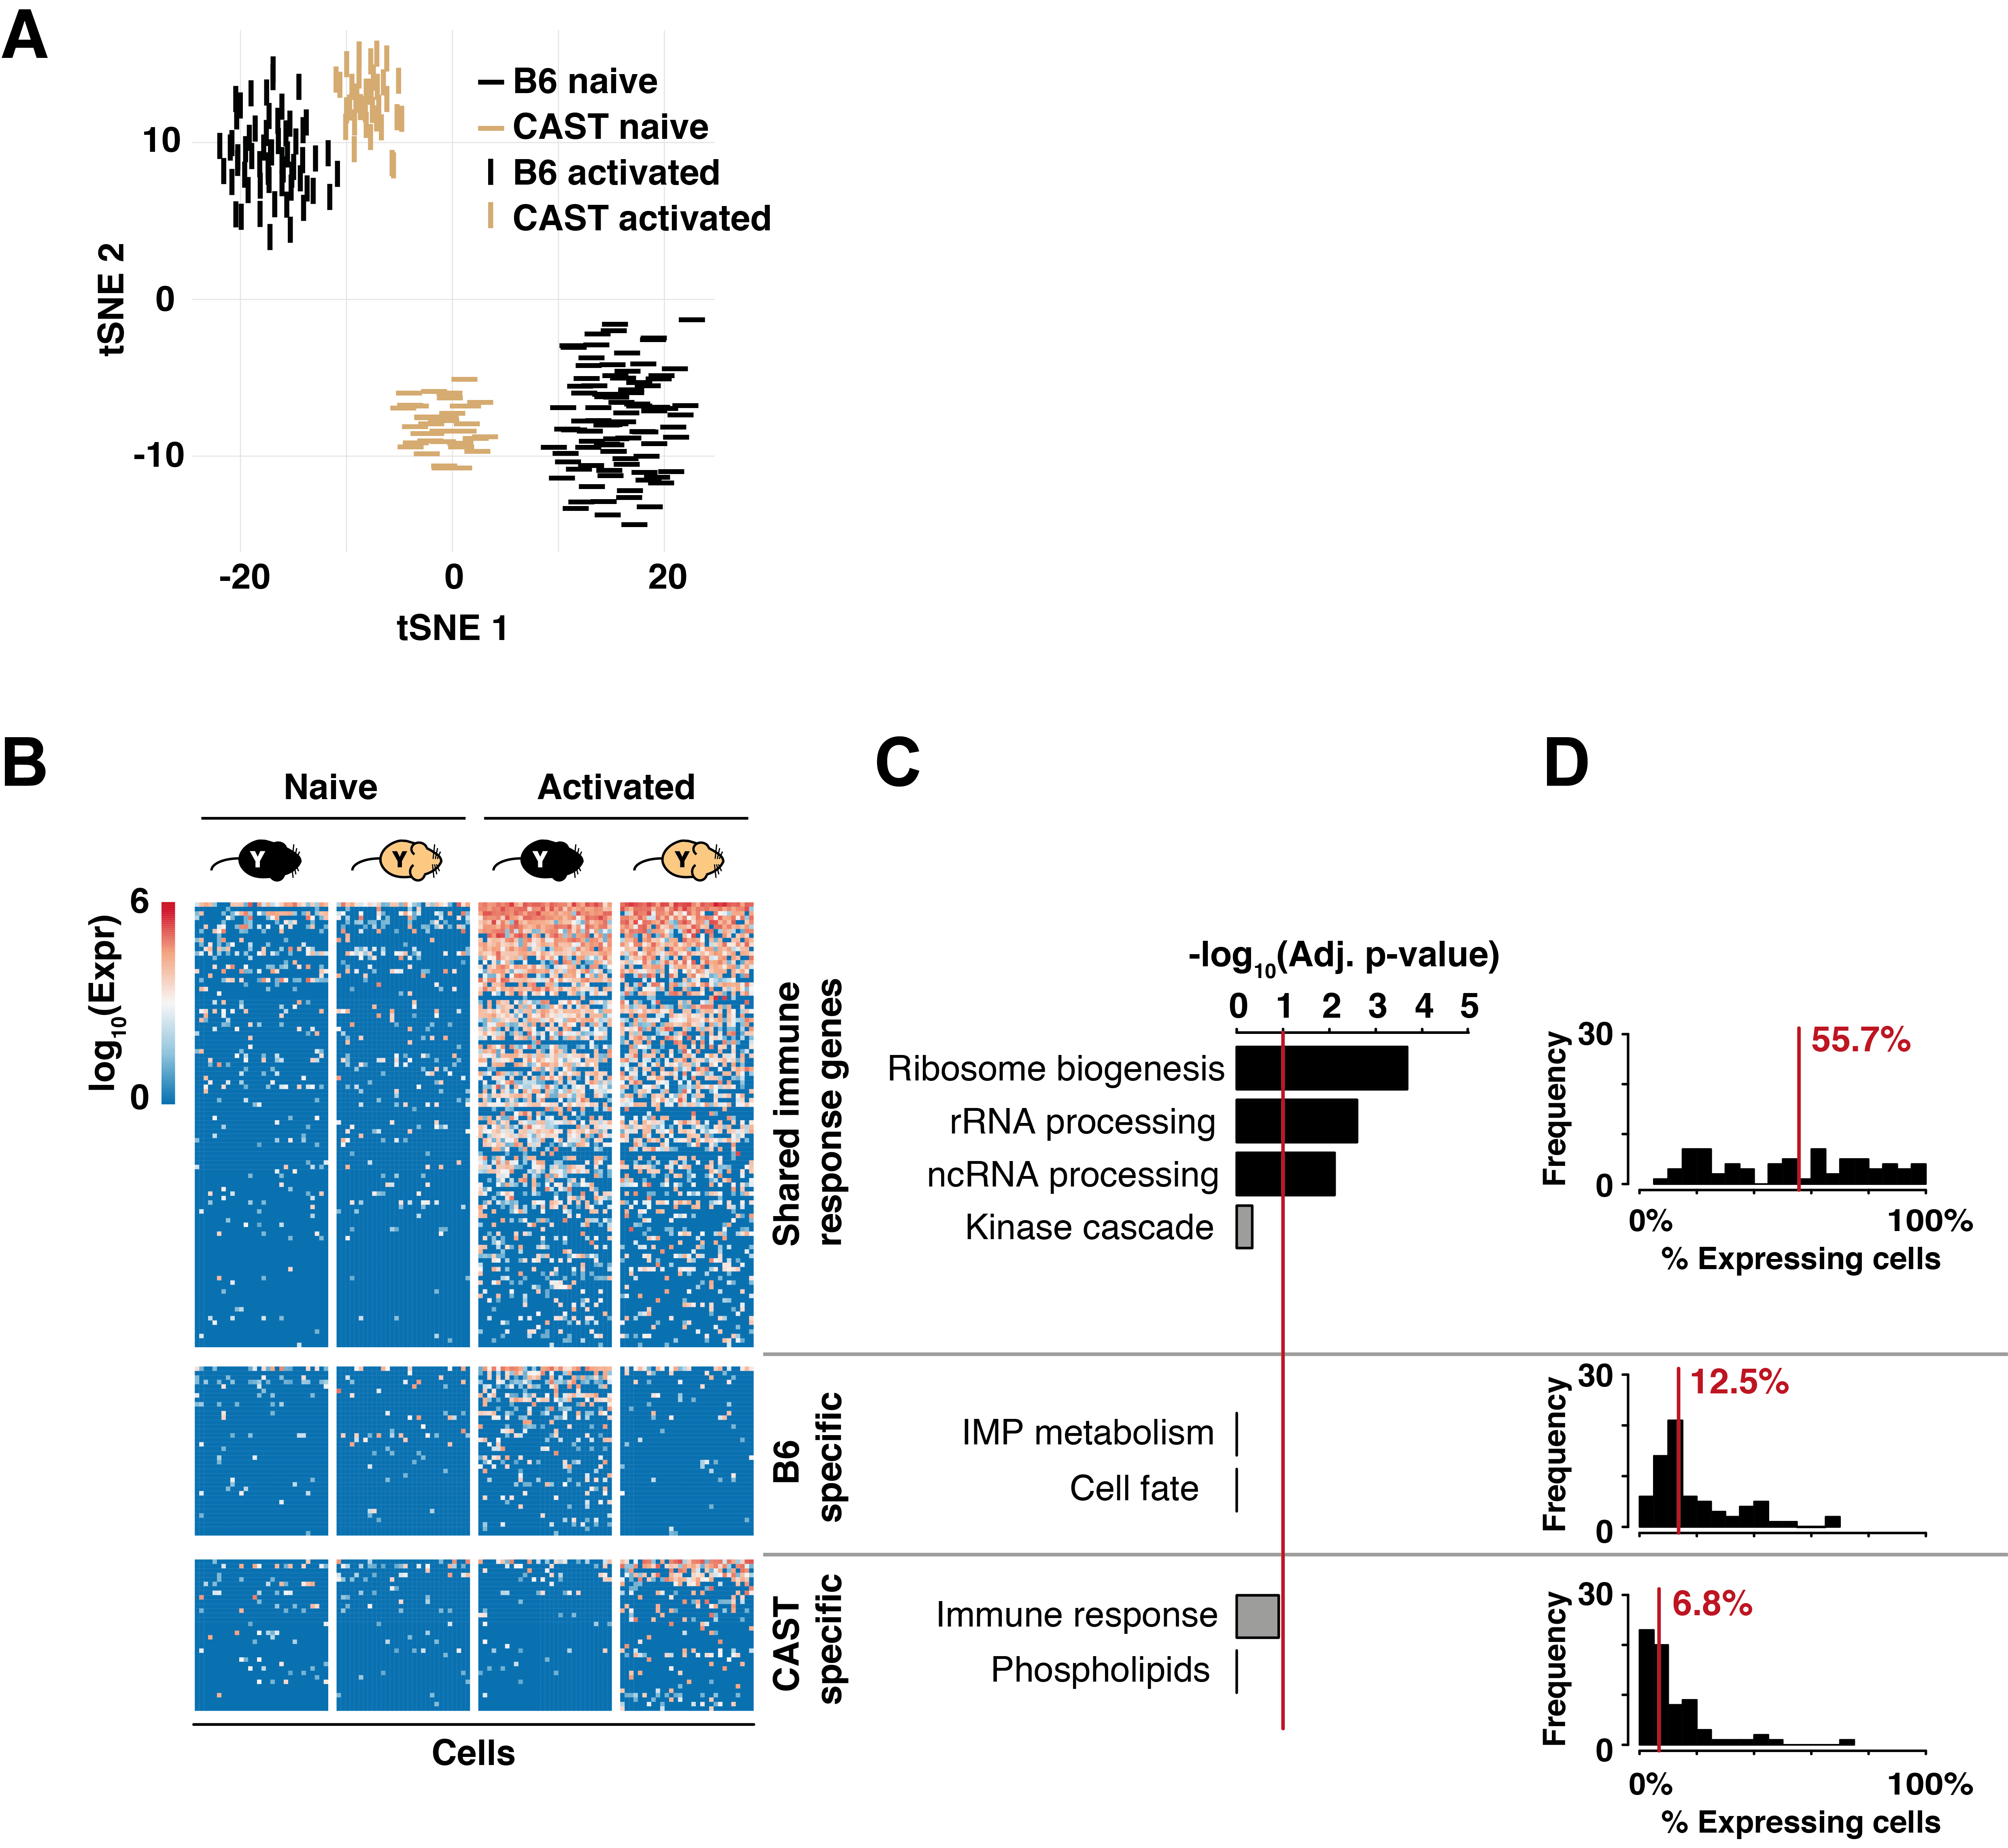
\includegraphics[width=\textwidth]{Fig_11.png}
\caption[Shared CD4\plus{} T cell activation programme]{\textbf{Shared CD4\plus{} T cell activation programme.}\\
\textbf{(A)} CD4\plus{} T cells isolated from B6 (black) and CAST (orange) show similar large-scale transcriptional changes upon immune stimulation, \textbf{(B)} Immune activation of CD4\plus{} T cells triggers up-regulation of both conserved (upper panel), and species-specific (lower panels) transcriptional programs. For visualisation purposes, genes in shared and species-specific categories were proportionately and randomly selected. 30 cells were randomly selected for each condition/species, \textbf{(C)} Genes up-regulated in both B6 and CAST highly enrich for known T cell functionality. Genes up-regulated in only B6 or CAST have no statistically significant functional enrichment (Bonferroni multiple testing corrected p-values, red line is 0.1), \textbf{(D)} Fractions of cells in which a gene is detected are displayed as histograms. 70 genes were randomly selected from each gene set. While most genes in the shared activation process are expressed in a high percentage of cells, only few cells express species-specific genes of the activation process. From \citep{Martinez-jimenez2017}. Reprinted with permission from AAAS.}
\label{fig1:shared_activation}
\end{figure}

\newpage

\subsection{Functional assessment of the conserved response genes}

We next estimated functionality of these 225 shared response genes by enrichment and variability analysis. Firstly, when performing GO analysis, the set of shared genes was strongly enriched for cellular processes known to be immediately activated by stimulation of CD4\plus{} T cells. This includes the core translational machinery (ribosome biogenesis and \glspl{rRNA}, \textbf{Fig.~\ref{fig1:shared_activation}C}) and key immune activation genes (such as \textit{Il2ra} and \textit{Tnfrsf9}, \citep{Asmal2003}). Other categories of immune response genes include cytokines, chemokines and their receptors (e.g.\textit{Ccr8}, \textit{Il2}, \textit{Ccl3}, \citep{Turner2014}), members of the \gls{Nr} superfamily (e.g. \textit{Nr4a2}, \textit{Nr4a3}, \textit{Nr4a1}, \citep{Glass2010}), components of NF$\kappa$B signalling (e.g. \textit{Nfkbid}, \textit{Nfkb1}, \textit{Nfkbie}, \textit{Rel}, \citep{Gerondakis2010}) and Tnf signalling (e.g. \textit{Tnf}, \textit{Tnfsf14}, \textit{Tnfrsf4}, \textit{Tnfrsf1b}, \citep{Croft2009}). In contrast, species-specific genes (96 for B6, 75 for CAST) showed no enrichment for biological function \textbf{(Fig. \ref{fig1:shared_activation}C)}. \\

As described in \textbf{Section \ref{sec1:species-spec-dynamics}}, the degree of heterogeneity to which genes are expressed within a homogeneous population of cells can indicate the functional relevance of these genes for population responses. We therefore calculated the fraction of cells that express shared and species-specific immune response genes (> 0 counts). Shared immune response genes were expressed across most CD4\plus{} T cells in both B6 and CAST after activation. In contrast, species-specific response genes tend to be expressed in a smaller fraction of cells \textbf{(Fig. \ref{fig1:shared_activation}D)}. \\

Our interspecies comparison thus revealed that target genes involved in translational control and immune function represent the conserved signature within the early activation response. These genes are furthermore similarly up-regulated in most cells across the homogeneous population of activated CD4\plus{} T cells. 

\newpage

\section{Destabilisation of CD4\plus{} T cell activation during ageing}

Ageing can cause perturbation of cell cycle entry for haematopoietic stem cells, leading to a shift in the functional balance between self-renewal and differentiation \citep{Kowalczyk2015}. We considered whether ageing might similarly perturb the transcriptional response of CD4\plus{} T cells to immune stimulation. For this, we performed differential expression and differential variability analysis between cells isolated from young and old animals. By comparing the activation responses between different sub-species of mice, we could also establish whether any observed impact of ageing is conserved. Lastly, we compare the effect of ageing across different subsets of CD4\plus{} T cells to assess how the effects of ageing differ across the immune system.

\subsection{Ageing does not effect CD4\plus{} T cell transcription on a global level}
\label{sec1:global_changes}

We first asked whether the overall response of CD4\plus{} T cells is perturbed during ageing. For this we (i) performed PCA and (ii) compared mean expression of cells isolated from young and old mice. PCA revealed that the global expression profiles of naive or activated CD4\plus{} T cells not heavily effected by ageing \textbf{(Fig.~\ref{fig1:mean_expression_ageing}A and B)}. Furthermore, we identified differentially expressed genes between young and old animals separately for naive and activated CD4\plus{} T cells \textbf{(Fig.~\ref{fig1:mean_expression_ageing}C and D)}. This analysis was performed separately for each species. Only around 10\% of all tested genes showed changes in mean expression between young and old animals. Additionally, these genes typically showed low expression in naive or activated cells taken from both young and old animals. To further quantify this, we computed the fraction of cells in which each differentially expressed gene was expressed. The distribution of these values was added as inlets to the plots in \textbf{Fig.~\ref{fig1:mean_expression_ageing}C and D} (x-axis ranging from 0\% to 100\% of cells). We detect that differentially expressed genes are enriched for those that are only expressed in subsets of cells. This indicates that changes in mean expression during ageing only affect lowly expressed genes that are detected only in subsets of cells and therefore do not contain functionally relevant genes. These effects can also arise due to increased levels of noise for lowly expressed genes \citep{Brennecke2013}. \\

Nevertheless, to test whether these subtle effects during ageing are shared between the two species, we calculated the Jaccard index, which measures the overlap between sets of elements, separately for up- and down-regulated genes \textbf{(Fig.~\ref{fig1:mean_expression_ageing}E and F)}. We only detect $\sim$3\% of the differentially expressed genes as being shared between the two species either for up-regulated genes or down-regulated genes during ageing. Therefore, we did not find a conserved ageing signature that affects expression levels in CD4\plus{} T cells.

\newpage

\begin{figure}[!ht]
\centering
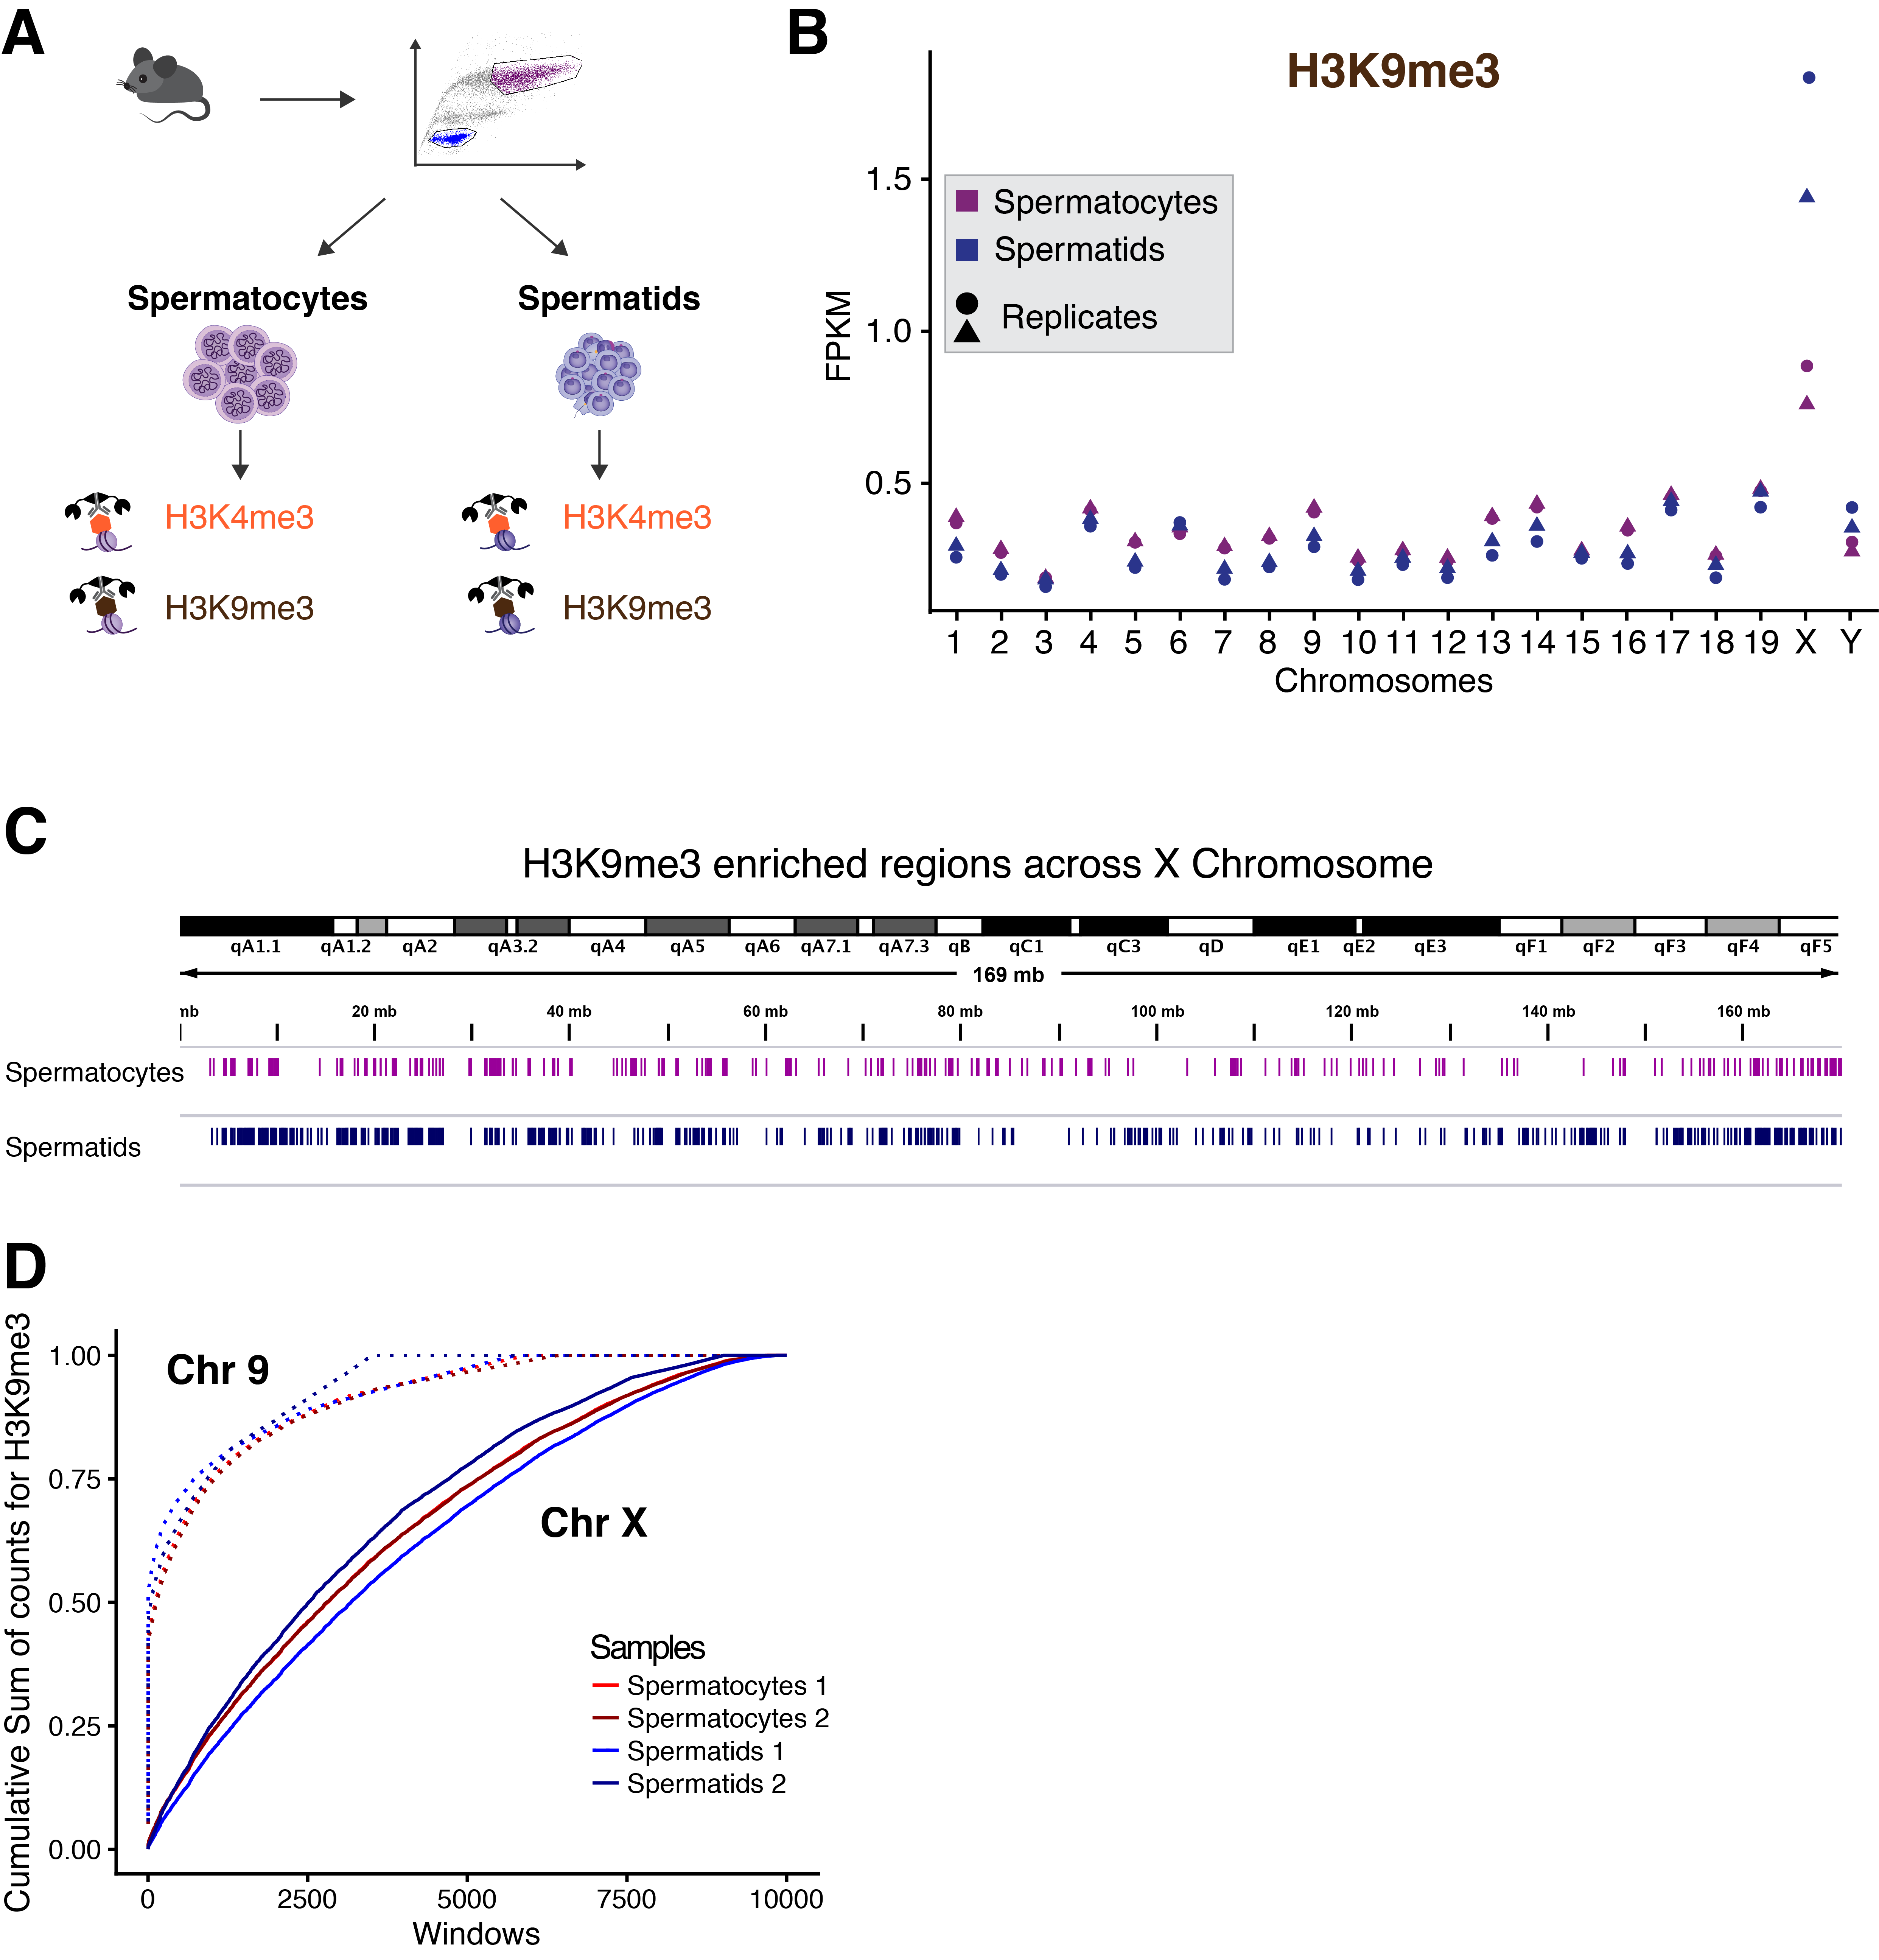
\includegraphics[width=0.9\textwidth]{Fig_12.png}
\caption[Global immune response during ageing]{\textbf{Ageing did not change the global expression profile of naive or activated CD4\plus{} T cells (full legend on next page).}}
\label{fig1:mean_expression_ageing}
\end{figure}

\newpage

\captionsetup[figure]{list=no}
\addtocounter{figure}{-1}   
\captionof{figure}{\textbf{Ageing did not change the global expression profile of naive or activated CD4\plus{} T cells (continued).}\\
Principal component analysis reveals no separation between cells isolated from young or old animals in the naive \textbf{(A)} or activated \textbf{(B)} state, \textbf{(C)} 7.1\% of all tested genes in B6 and 10.3\% of genes in CAST are differentially expressed in naive CD4\plus{} T cells between old (red) and young (blue) animals. Average gene expression using posterior estimation, threshold of means > 50, log2FC in $\mu_i$ > 2, EFDR = 5\%. Insets show distributions of fraction of cells in which these genes are expressed. X-axis: 0\% - 100\% of cells,  \textbf{(D)} 10\% of all tested genes in B6 and 9\% of genes in CAST are differentially expressed in activated CD4\plus{} T cells between old (red) and young (blue) animals. Average gene expression using posterior estimation, threshold of means > 50, log2FC in $\mu_i$ > 2, EFDR = 5\%. Insets show distributions of fraction of cells in which these genes are expressed. X-axis: 0\% - 100\% of cells, \textbf{(E)-(F)} The overlap of ageing-associated genes in \textbf{(E)} naive or \textbf{(F)} activated cells was calculated using the Jaccard index between gene sets. Genes highly expressed in old animals (red) or genes highly expressed in young animals (blue) show little overlap (2-3\%) between B6 and CAST. From \citep{Martinez-jimenez2017}. Reprinted with permission from AAAS.
\\}
\captionsetup[figure]{list=yes}

\subsection{Ageing increases transcriptional variability in response genes}

To further dissect possible ageing effects on the core functionality of CD4\plus{} T cells, we next focused on the conserved activation program.
This analysis is more targeted and allows us to detect more subtle changes caused by ageing. Qualitatively, and consistent with the findings in \textbf{Section \ref{sec1:global_changes}}, the majority of genes in the core activation program responded upon stimulation, irrespective of age \textbf{(Fig.~\ref{fig1:variability_ageing}A)}. We then profiled changes in mean expression of activated cells between young and old animals for both species. This analysis resulted in a subtle decrease in expression for aged individuals while the majority of genes showed similar expression between young and old, as expected \textbf{(Fig.~\ref{fig1:variability_ageing}B)}. \\

We next profiled changes in variability by considering genes with no changes in mean expression in activated cells between between young and old animals (see \textbf{Section \ref{sec1:computational}}). By plotting the log2FC in $\delta_i$ for these genes, we observe an increase in cell-to-cell transcriptional variability of the core activation program in older animals compared to young animals \textbf{(Fig. \ref{fig1:variability_ageing}C)}. To identify the drivers of the increase in transcriptional variability of the immune response during ageing, we calculated the fraction of activated cells in which genes of the shared activation program are expressed. By comparing these fractions between activated cells isolated from old or young animals in both species, we identify consistently fewer cells from aged animals that express the shared activation programme \textbf{(Fig. \ref{fig1:variability_ageing}D)}. \\

\newpage

\begin{figure}[!ht]
\centering
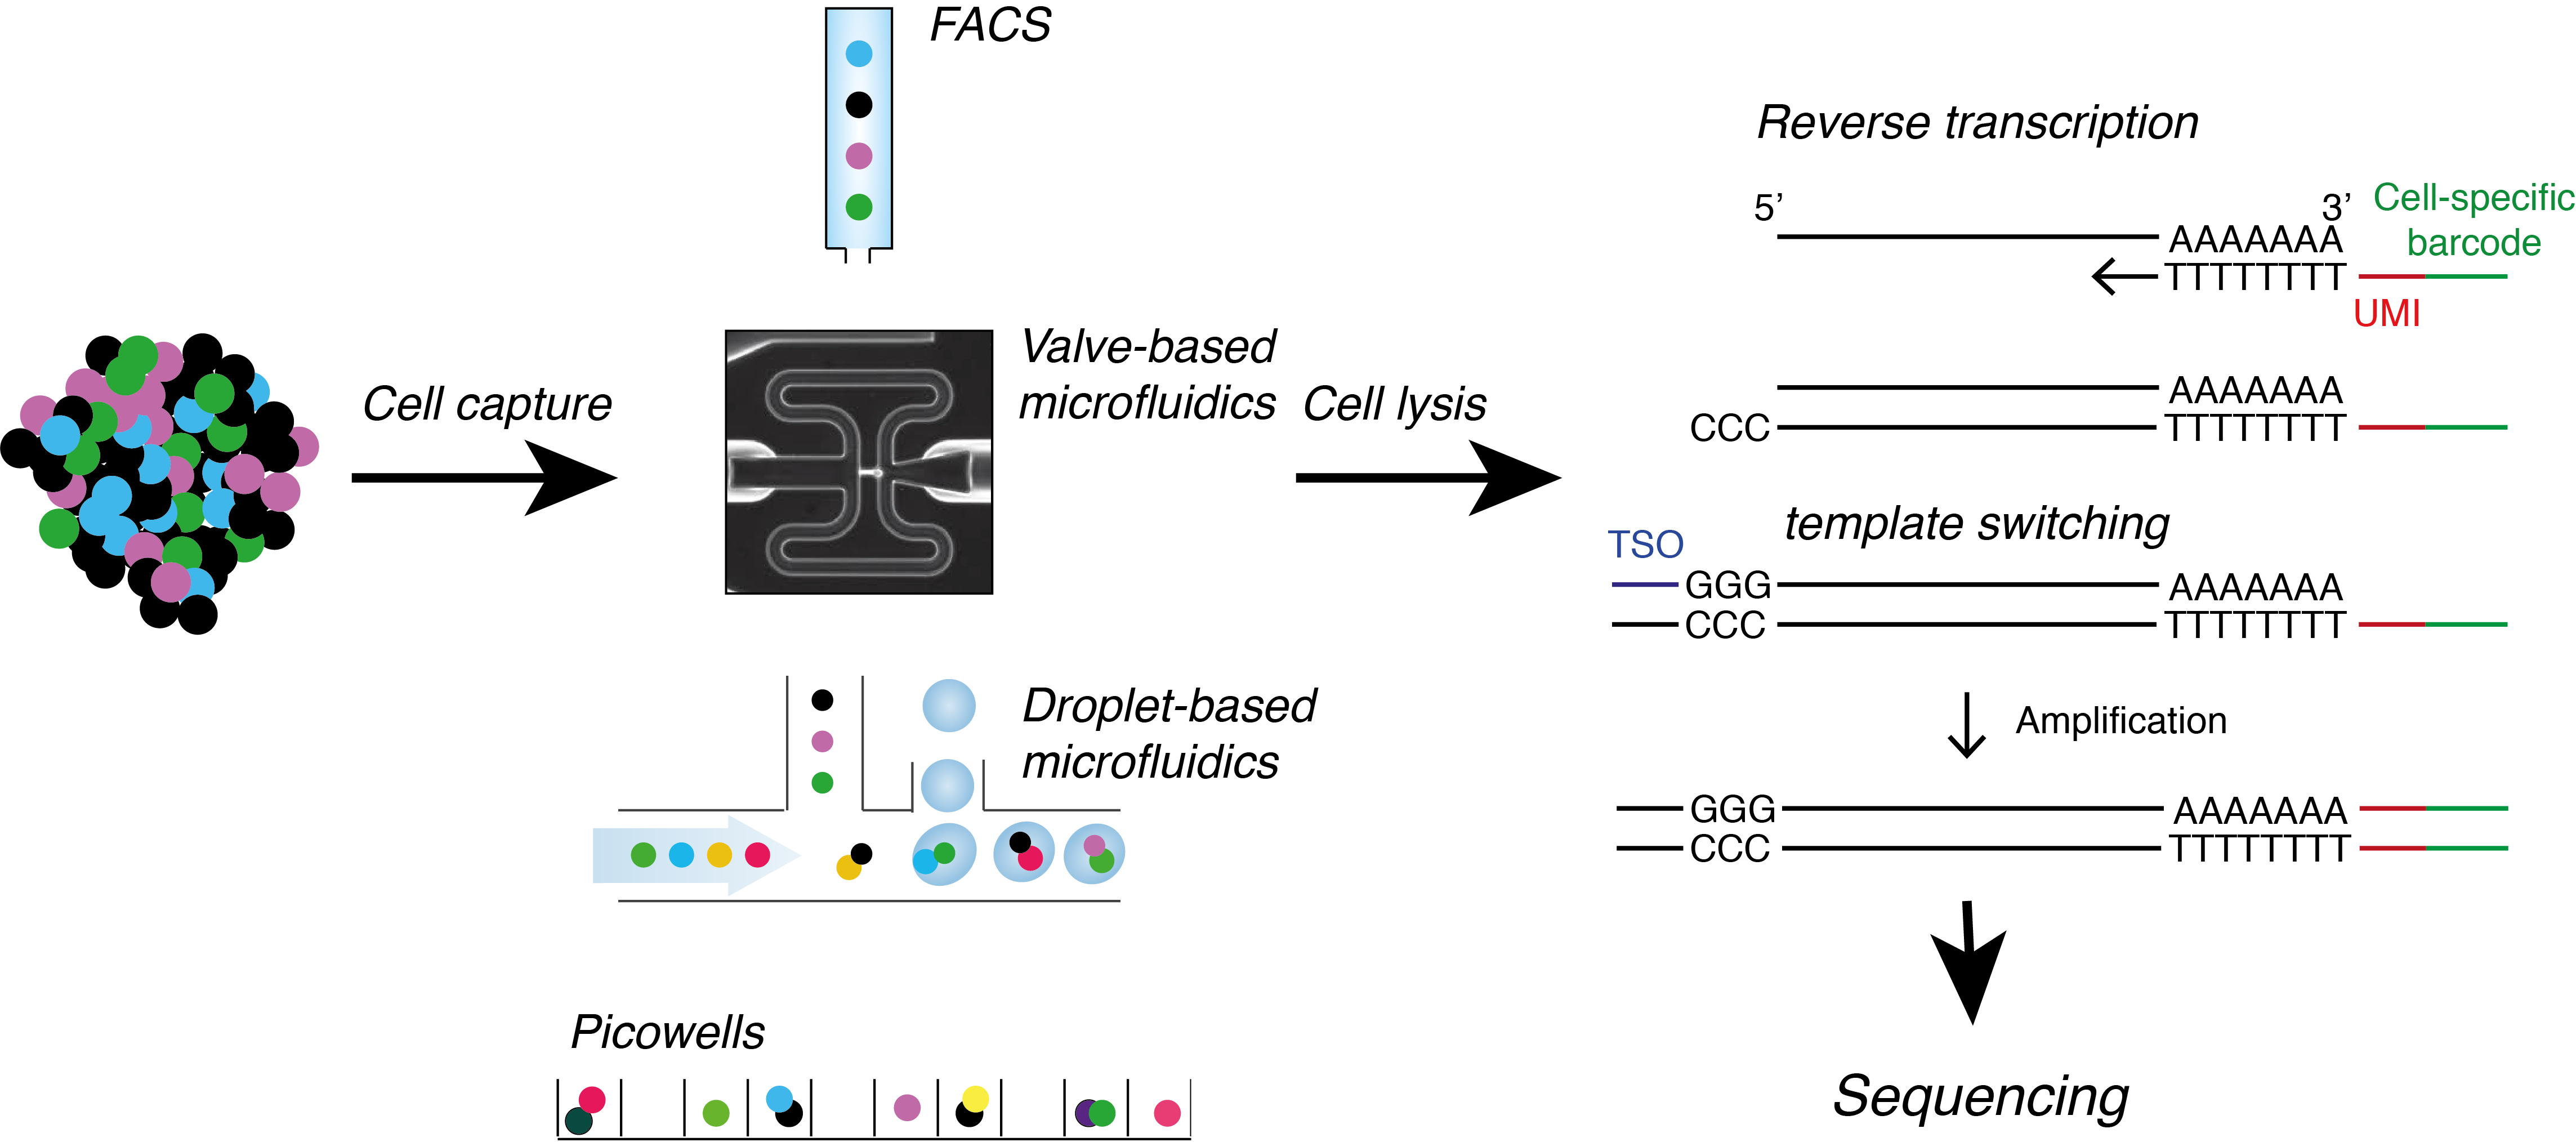
\includegraphics[width=\textwidth]{Fig_13.png}
\caption[Ageing destabilises the CD4\plus{} T cell response]{\textbf{Ageing destabilises the CD4\plus{} T cell response.} \\
\textbf{(A)} Full heatmap showing all 225 genes of the shared activation program expressed in all activated cells from young and old CAST and B6. Genes were ordered based on their mean expression, \textbf{(B)} Fold changes in mean expression indicate a consistent trend in lower expression of the shared activation program in cells from old animals (genes were ordered by mean expression, log2FC of posterior mean estimates), \textbf{(C)} Cells from old animals show higher transcriptional variability compared to young animals (genes were ordered by mean expression, log2FC of posterior over-dispersion estimates), \textbf{(D)} The fraction of cells in which genes of the shared activation process are expressed is reduced in activated CD4\plus{} T cells from old animals. The distribution of fraction values is plotted on each corresponding axis (medians of fraction values are indicated in red); statistically significant changes in the percentage of cells expressing genes of the core activation process were assessed using a binomial test (blue points indicate bonferroni corrected p-values < 0.1). Gene expression in activated cells isolated from old animals was used as the Null-distribution.}
\label{fig1:variability_ageing}
\end{figure}

\newpage

These results indicate a destabilisation of the immune response programme during ageing. While most response genes are expressed at similar levels in activated cells of young and old animals, we detect a subset of cells where the expression of these genes is lost in aged mice. These dropouts in expression do not correlate across the population of cells and appear to be more stochastic. 

\subsection{Validation experiments to confirm changes in variability}

We next asked whether the increase in variability is driven by (i) technical factors, (ii) biases in model parameter estimation or (iii) hidden sub-structure within the data. To address the first point, we generated independent replicates of naive and activated CD4\plus{} T cells from young and old B6 animals using Fluidigm C1 machines located at a different research institute. Profiling changes in variability using these biological replicates, we validated the increase in transcriptional variability during ageing \textbf{(Fig. \ref{fig1:validation}A)}.\\

Secondly, quantification of transcriptional variability can be biased based on the number of cells present in each cell population. When assaying homogeneous cell populations with larger sample size, model parameter estimation is more precise compared to populations with smaller sample size (see \textbf{Section \ref{sec2:stabilization}}). We therefore downsampled both young and old activated CD4\plus{} T cells to equal size and detected the same increase in variability during ageing \textbf{(Fig.~\ref{fig1:validation}B)} as previously when comparing the full set of CD4\plus{} T cells \textbf{(Fig.~\ref{fig1:variability_ageing}C)}. \\

Thirdly, in \textbf{Section \ref{sec1:characterization}} we observed that old animals have a small population of CD4\plus{} T cells with slightly elevated CD44 levels, reduced CD62L expression, and attenuated activation dynamics \textbf{(Fig.~\ref{fig1:characterization}E-G)}. We therefore tested whether the global shift in variability is caused by different cell population structures between old and young B6 animals. To that end, cells expressing marker genes that were inconsistent with their activation state as well as cells with a possible Th1 differentiation bias (\textit{Ifng} expressing) were removed. Based on the library size adjusted counts, we removed activated cells with low \textit{Cd69} (< 300 counts), high \textit{Sell} (> 10 counts), low \textit{Trac} (< 100 counts), low \textit{Il2ra} (< 100 counts) and \textit{Ifng} (> 0 counts) expression \textbf{(Fig. \ref{fig1:validation}C)}. The remaining 37 and 26 activated cells in young and old B6 animals showed the same shift in transcriptional variability compared to the non-filtered data \textbf{(Fig. \ref{fig1:validation}D)}. 

\newpage

\begin{figure}[!ht]
\centering
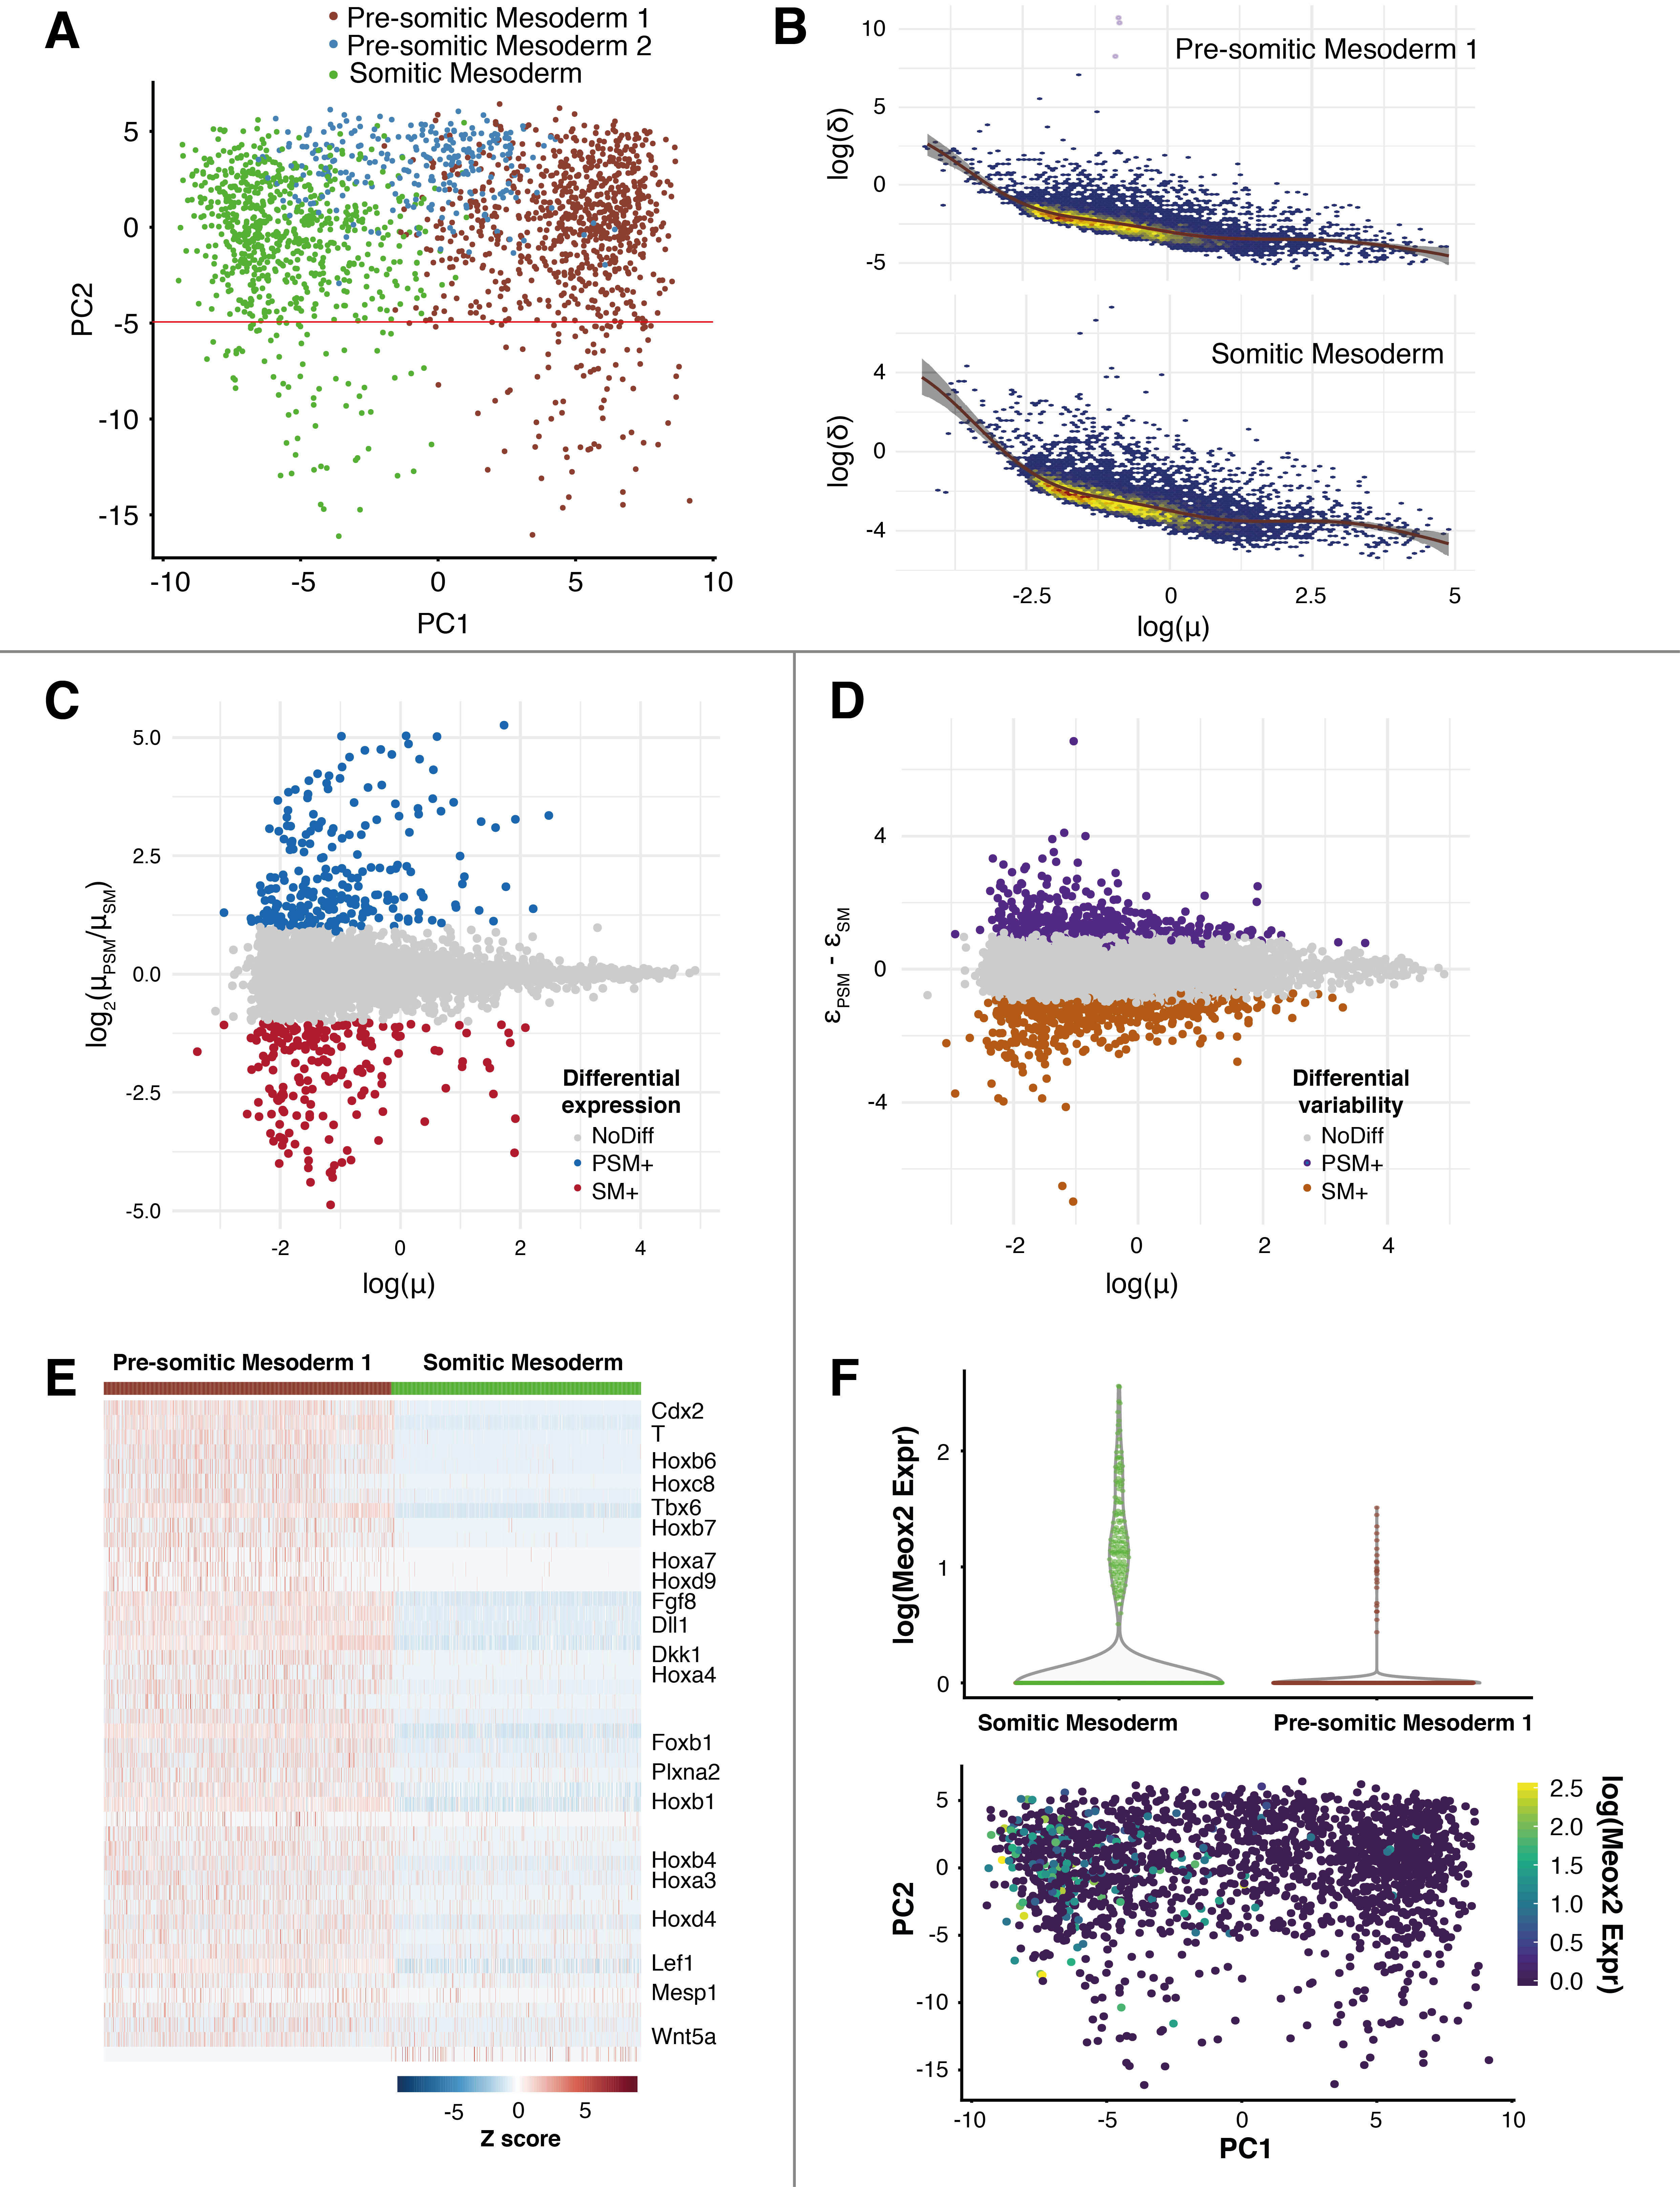
\includegraphics[width=\textwidth]{Fig_14.png}
\caption[Experimental validation of increased transcriptional variability during ageing]{\textbf{Experimental validation of increased transcriptional variability during ageing.} \\
\textbf{(A)} A biological replicate of 115 activated CD4\plus{} T cells from old B6 animals was generated and changes in gene expression variability were compared to activated CD4\plus{} T cells from young B6 animals, \textbf{(B)} 30 out of all activated CD4\plus{} T cells from young or old B6 mice were randomly selected and changes in gene expression variability were compared between the downsampled populations of cells, \textbf{(C)} Expression of CD4\plus{} T cell activation markers in all activated cells from young and old B6 before (left) and after (right) filtering based on \textit{Ifng}, \textit{Sell}, \textit{Trac}, \textit{Il2ra} and \textit{Cd69} expression, \textbf{(D)} Changes in gene expression variability of activated cells between young and old animals are displayed before (left) and after (right) filtering (see (C)).}
\label{fig1:validation}
\end{figure}

\newpage

\subsection{Transcriptional variability in CD4\plus{} T cell subsets}

It is well known that T cell-type composition changes are driven by thymic involution which leads to a reduction of the thymic output in CD4\plus{} T cells over age. After infections, previously activated CD4\plus{} T cells survive and form central memory T cells \cite{Moro-Garcia2013}.\\

We first address if the decrease in thymic output over age induces a reduction of \glspl{RTE} in the spleen and therefore biases expression variability to be higher in aged animals. Maturation of RTEs contributes significantly to the maintenance of the naive CD4\plus{} T cell pool in the periphery and is affected by ageing \citep{Boursalian2004, Hale2006, Fink2013}. To estimate proportions of RTEs within the naive CD4\plus{} T cell pool, we characterised CD4 single positive (SP) thymocytes and splenic naive CD4\plus{} T cells by flow cytometry. RTEs can be identified by their CD24$^{\text{hi}}$ Qa2$^{\text{lo}}$ phenotype \citep{Boursalian2004, Hale2006}. We find the  majority of CD4 SP thymocytes showed a CD24$^\text{hi}$ Qa2$^\text{lo}$ phenotype \textbf{(Fig.~\ref{fig1:EM_Naive_CD4}A)}. In contrast, we detected only a very small population of RTEs (~2\%) within splenic naive CD4\plus{} T cell pool similarly in young and old mice \textbf{(Fig.~\ref{fig1:EM_Naive_CD4}A and B)} \citep{Hale2006}. This suggests minimal contamination of RTEs in naive CD4\plus{} T cells purified by MACS and therefore no bias when testing for changes in variability.\\

Next, we examine whether the age-mediated increase in cell-to-cell variability is conserved across different subsets of CD4\plus{} T cells. We therefore sorted naive and EM CD4\plus{} T cells as explained in \textbf{Fig.~\ref{fig1:FACS}}. We detect the decline in naive CD4\plus{} T cells and an enrichment of EM CD4\plus{} T cells in old animals. Furthermore, and as expected, we identify a significantly higher proportion of EM CD4\plus{} T cells in old animals that express the activation markers CD69 and PD-1, indicating that a larger fraction of cells is already in an activated state \textbf{(Fig. \ref{fig1:EM_Naive_CD4}C)}. To avoid this phenomenon to interfere with the quantification of transcriptional variability, cells stained positive for CD69 and/or PD-1 were excluded during the sort of EM CD4\plus{} T cells by FACS. After sorting, we compared transcriptional variability of the core set of immune response genes in activated cells between old and young animals. Critically, these genes showed an increase in variability in older animals in both FACS-purified naive and EM CD4\plus{} T cell subsets similar to MACS-purified cells  \textbf{(Fig.~\ref{fig1:EM_Naive_CD4}D and E)}.\\

To conclude, ageing reduces the fraction of cells in which immune activation genes are up-regulated, thus increasing cell-to-cell heterogeneity and attenuating the response to stimulation across multiple CD4\plus{} T cell subsets.

\newpage

\begin{figure}[!ht]
\centering
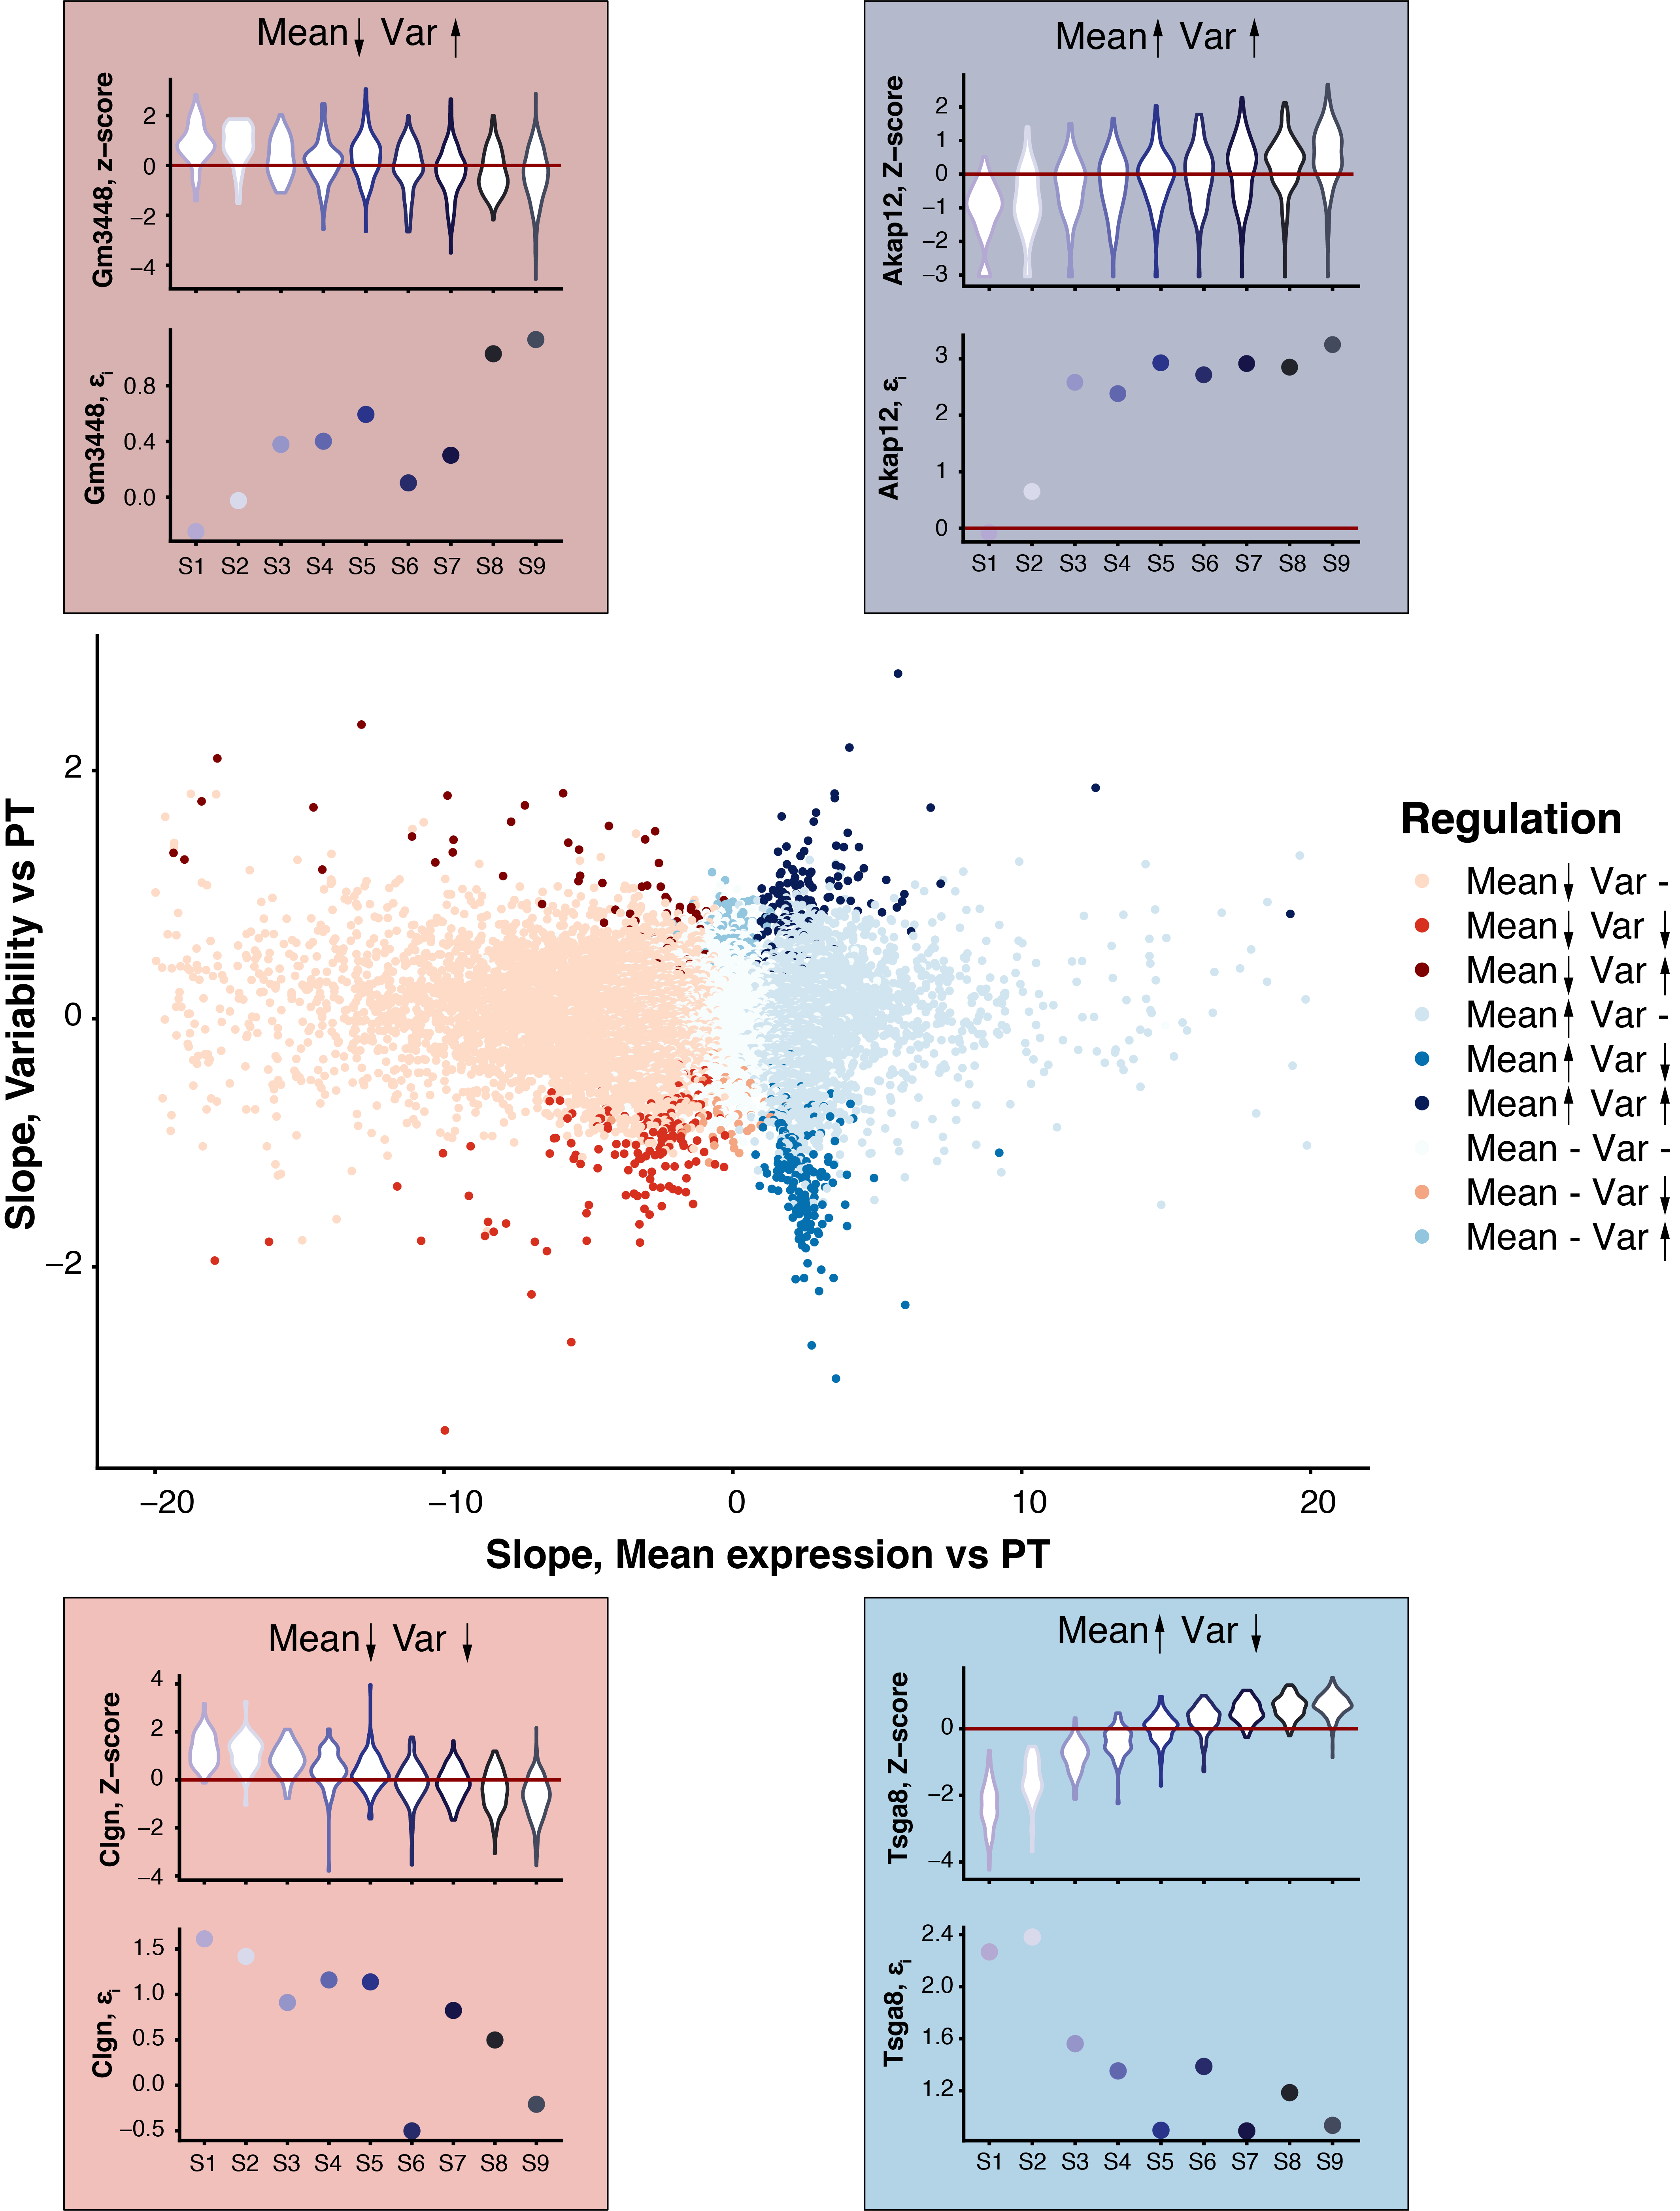
\includegraphics[width=\textwidth]{Fig_15.png}
\caption[Increased expression variability during ageing in different CD4\plus{} T cell subsets]{\textbf{Increased expression variability during ageing in different CD4\plus{} T cell subsets.} \\
\textbf{(A)} Thymus and spleen were collected from young and old B6 mice, dissociated into single cell suspensions, stained with viability dye and antibodies against CD4, CD8, CD24 and Qa2 for thymocytes or antibodies against CD4, CD44, CD62L, CD24 and Qa2 for splenocytes. FACS plots shown are gated on single, live cells and either CD4\plus{} CD8\textsuperscript{-} CD4 \gls{SP} thymocytes (thymus) or CD44$^\text{lo}$ CD62L$^\text{hi}$ naive CD4\plus{} T cells (spleen). Percentages relate to total gated cells. In the thymus the majority of CD4 SP express markers of recent thymic emigrants (RTEs, CD24$^\text{hi}$ Qa2$^\text{lo}$) while in the spleen naive CD4\plus{} T cells are comprised mainly of mature naive cells (red box), \textbf{(B)} Quantification of flow cytometry data from (A). Significance of difference was calculated by Mann-Whitney test (ns = not significant). MNT = mature naive T cell, \textbf{(C)} Spleens were collected from young and old B6 mice, dissociated into single cell suspensions, stained with viability dye and antibodies against CD4, CD44, CD62L, CD24, Qa2, CD69, and PD-1. FACS plots were gated on single, live, CD4\plus{} T cells and subsequently on either CD44$^\text{lo}$ CD62L$^\text{hi}$ (Naive) or CD44$^\text{hi}$ CD62L$^\text{lo}$ (EM) subsets. Expression of CD69 and PD-1 was analysed in these subsets. Results shown are pooled from 10 independent experiments with spleens harvested from 5 young and 5 old mice. Significance of difference was calculated by two-way ANOVA ($^{\ast{}\ast{}\ast{}\ast}$p $\leq$ 0.0001); \textbf{(D)} Activated, FACS-purified naive CD4\plus{} T cells from old animals showed higher transcriptional variability compared to young animals, \textbf{(E)} Activated, FACS-purified EM CD4\plus{} T cells from old animals showed higher transcriptional variability compared to young animals.}
\label{fig1:EM_Naive_CD4}
\end{figure}

